%\documentclass[12pt]{aastex}
\documentclass[iop]{emulateapj}
%\documentclass{article}
%\usepackage{draftwatermark}
\usepackage{paralist}
\shorttitle{Magnetized massive disks}
\shortauthors{M-K. Lin}

\usepackage{amsmath}
%\usepackage{url}
\usepackage{bm}
%\usepackage[font=small,format=plain,labelfont=bf,up,textfont=it,up]{caption}
\newcommand{\p}{\partial}
\newcommand{\lmax}{l_\mathrm{max}}
\newcommand{\sbar}{\bar{\sigma}} 
\newcommand{\imgi}{\mathrm{i}} 
\newcommand{\ii}{\mathrm{i}}
\newcommand{\C}{\mathcal{C}^\lambda}
\newcommand{\wop}[1]{\mathcal{V}^{(#1)}}
\newcommand{\avg}[1]{\langle{#1}\rangle}
\newcommand{\zhat}{\hat{z}}
\newcommand{\rhat}{\hat{r}}
\newcommand{\he}{\mathcal{H}}
\newcommand{\amp}{\mathcal{A}}
\newcommand{\dd}{\delta}
\newcommand{\real}{\operatorname{Re}}
\newcommand{\imag}{\operatorname{Im}}
\newcommand{\sgn}{\operatorname{sgn}}
\newcommand{\zmax}{Z_s}
\newcommand{\wbar}{\tilde{W}}
\newcommand{\qbar}{\tilde{Q}}
\newcommand{\dbigH}{\frac{H^\prime}{H}}
\newcommand{\Rp}{\frac{\rho_0^\prime}{\rho_0}}
\newcommand{\Fp}{\frac{g^\prime}{g}}
\newcommand{\Rpp}{\frac{\rho_0^{\prime\prime}}{\rho_0}}
\newcommand{\Fpp}{\frac{g^{\prime\prime}}{g}}
\newcommand{\ils}{L_s^{-1}}
\newcommand{\ilp}{L_p^{-1}}
\newcommand{\ihp}{H_p^{-1}}
\newcommand{\ihs}{H_s^{-1}}
\newcommand{\ciso}{c_\mathrm{iso}}
\newcommand{\csmid}{c_{s0}} 
\newcommand{\hiso}{h_\mathrm{iso}}
\newcommand{\Hiso}{H_\mathrm{iso}}
\newcommand{\zeus}{\texttt{ZEUS-MP }}
\newcommand{\rsph}{r_\mathrm{sph}}
\newcommand{\dvx}{\dd v_x}
\newcommand{\dvy}{\dd v_y}
\newcommand{\dvz}{\dd v_z}
\newcommand{\dbx}{\dd B_x}
\newcommand{\dby}{\dd B_y}
\newcommand{\dbz}{\dd B_z}
\newcommand{\w}{ \widetilde{W}}
%\newcommand{\sbar}{\bar{\sigma}}
\newcommand{\dphi}{\dd \Phi}
\defcitealias{lin12}{L12} 

\begin{document}

\title{Linear stability of magnetized massive protoplanetary disks}


\author{Min-Kai Lin (+Menou, Fromang, Youdin)}
\affil{Canadian Institute for Theoretical Astrophysics,
  60 St. George Street, Toronto, ON, M5S 3H8, Canada}
\email{mklin924@cita.utoronto.ca}

\begin{abstract}

\end{abstract}

\section{Introduction}
Understanding the evolution of protoplanetatry disks (PPDs) is key to
planet formation theory. A central aspect of PPD evolution is the mechanism
of angular momentum transport. It is believed that 



%early phases

%'dead zones'

%gi planet formation

%mri self-gravitating disks -> situations when mri is compressible 




\section{Local disk model}\label{setup}
We study the local stability of an inviscid, self-gravitating and
magnetized fluid disk orbiting a central star with
potential $\Phi_*(r,z)$, where $(r,\varphi,z)$ are cylindrical
co-ordinates from the star. We use the shearing box approximation     
\citep{goldreich65b} to consider a small patch of the disk at
a fiducial radius $r=r_0$. The local frame rotates at angular velocity 
$\Omega_0=\Omega(r_0,0)$ about the star, where $r\Omega^2 =
\p\Phi_*/\p r$. We also define $S\equiv-r\p\Omega/\p r$ as the local shear
rate and $\Omega_z^2\equiv\p^2\Phi_*/\p z^2$ as the square of the
local vertical frequency. 

A Cartesian co-ordinate system $(x,y,z)$ is set
up in this local frame, corresponding to the radial, azimuthal and vertical
directions of the global disk, respectively. The shearing box fluid
equations read 
\begin{align} 
  &\frac{\p\rho}{\p t}+\nabla\cdot(\rho\bm{v}) = 0,\\
  &\frac{\p \bm{v}}{\p t} + \bm{v}\cdot\nabla\bm{v} +
  2\Omega_0\hat{\bm{z}}\times\bm{v} = - \frac{1}{\rho}\nabla\Pi +
  \frac{1}{\rho\mu_0}\bm{B}\cdot\nabla\bm{B}
  -\nabla\Phi,\\
  &\frac{\p\bm{B}}{\p t}= \nabla\times\left(\bm{v}\times\bm{B} -
  \eta\nabla\times\bm{B}\right), 
\end{align}
where $\rho$ is the density field; $\bm{v}$ is the total velocity in
the local frame; $\bm{B}$ is the magnetic field which satisfies
$\nabla\cdot~\bm{B}=0$; $\Pi \equiv P +
|\bm{B}|^2/2\mu_0$ is the total pressure, and $\mu_0$ is the vacuum
permeability. We choose a barotropic equation of state, specified
below, so that the gas pressure is given by $P=P(\rho)$. The
resistivity $\eta$ is either uniform or a prescribed function of
height. 


The total potential is $\Phi = \Phi_\mathrm{ext} + \Phi_d$, where
\begin{align}
  \Phi_\mathrm{ext}(x,z) = -\Omega_0 S_0 x^2 +
  \frac{1}{2}\Omega_{z0}^2z^2 
\end{align}
is the effective external potential (central plus centrifugal) in the
shearing box approximation, where $S_0\equiv ~S(r_0,0)$ and
$\Omega_{z0}\equiv\Omega_z(r_0,0)$; 
and the gas potential $\Phi_d$ satisfies Poisson's equation
\begin{align}
  \nabla^2\Phi_d = 4\pi G \rho, 
\end{align}
where $G$ is the gravitational constant. For clarity, hereafter we
drop the subscript $0$ on the frequencies. 



\subsection{Equilibrium disk} 
The unperturbed disk is steady and described by
$\rho=~\rho(z)$, $\bm{B} = B_z\hat{\bm{z}} + B_y\hat{\bm{y}}$ where
$B_{y,z}$ are constants and the toroidal field strength is
$B_y=\epsilon B_z$. The equilibrium 
velocity field is $\bm{v} = -Sx\hat{\bm{y}}$. We consider Keplerian
disks so that $S = 3\Omega/2$ and the epicycle frequency 
$\kappa\equiv\sqrt{2\Omega(2\Omega-S)}=\Omega=\Omega_z$.  
We assume a thin disk and neglect the radial component of the
self-gravitational force in the unperturbed disk.    

The equilibrium density field is obtained by solving
\begin{align}
  &0=\frac{1}{\rho}\frac{d P}{dz} + \Omega_z^2z + \frac{d\Phi_d}{dz},\label{eqm_eqns1}\\
  &\frac{d^2\Phi_d}{dz^2} = 4\pi G \rho.\label{eqm_eqns2}
\end{align}
We consider \begin{inparaenum}[(i)]
\item isothermal disks with $P=c_{s0}^2\rho$\label{iso_eos}; 
\item polytropic disks with $P=K\rho^2$ with $K=c_{s0}^2/2\rho_0$;
\end{inparaenum}
where $\rho_0\equiv\rho(0)$ is the midplane density.
The sound speed $c_s\equiv\sqrt{dP/d\rho}$ 
so that $c_{s0}$ is the global sound speed in the isothermal disk, and
is the midplane sound speed in the polytropic disk. For the polytropic
disk the disk thickness $H$ is such that $\rho(H)=0$. Since the
isothermal disk has no surface, we define $H$ such that
$\rho(H)=10^{-2}\rho_0$. A non-dimensional
measure of the disk thickness is given by 
\begin{align}
  f^{-1} = \frac{H\Omega}{\csmid}, 
\end{align}
and $f$ will appear in subsequent discussions. 


We solve for $\hat{\rho}\equiv\rho/\rho_0$ with 
boundary conditions $\hat{\rho}=1$ and $d\hat{\rho}/dz=0$  at $z=0$. This
is done numerically for isothermal disks and analytically for the
polytropic disk (see Appendix \ref{appen1}). Examples of density
profiles are shown in Fig. \ref{eqm_den}. The normalized density field
is weakly dependent on the strength of self-gravity provided the
$z$-axis is appropriately scaled. 


\begin{figure}
  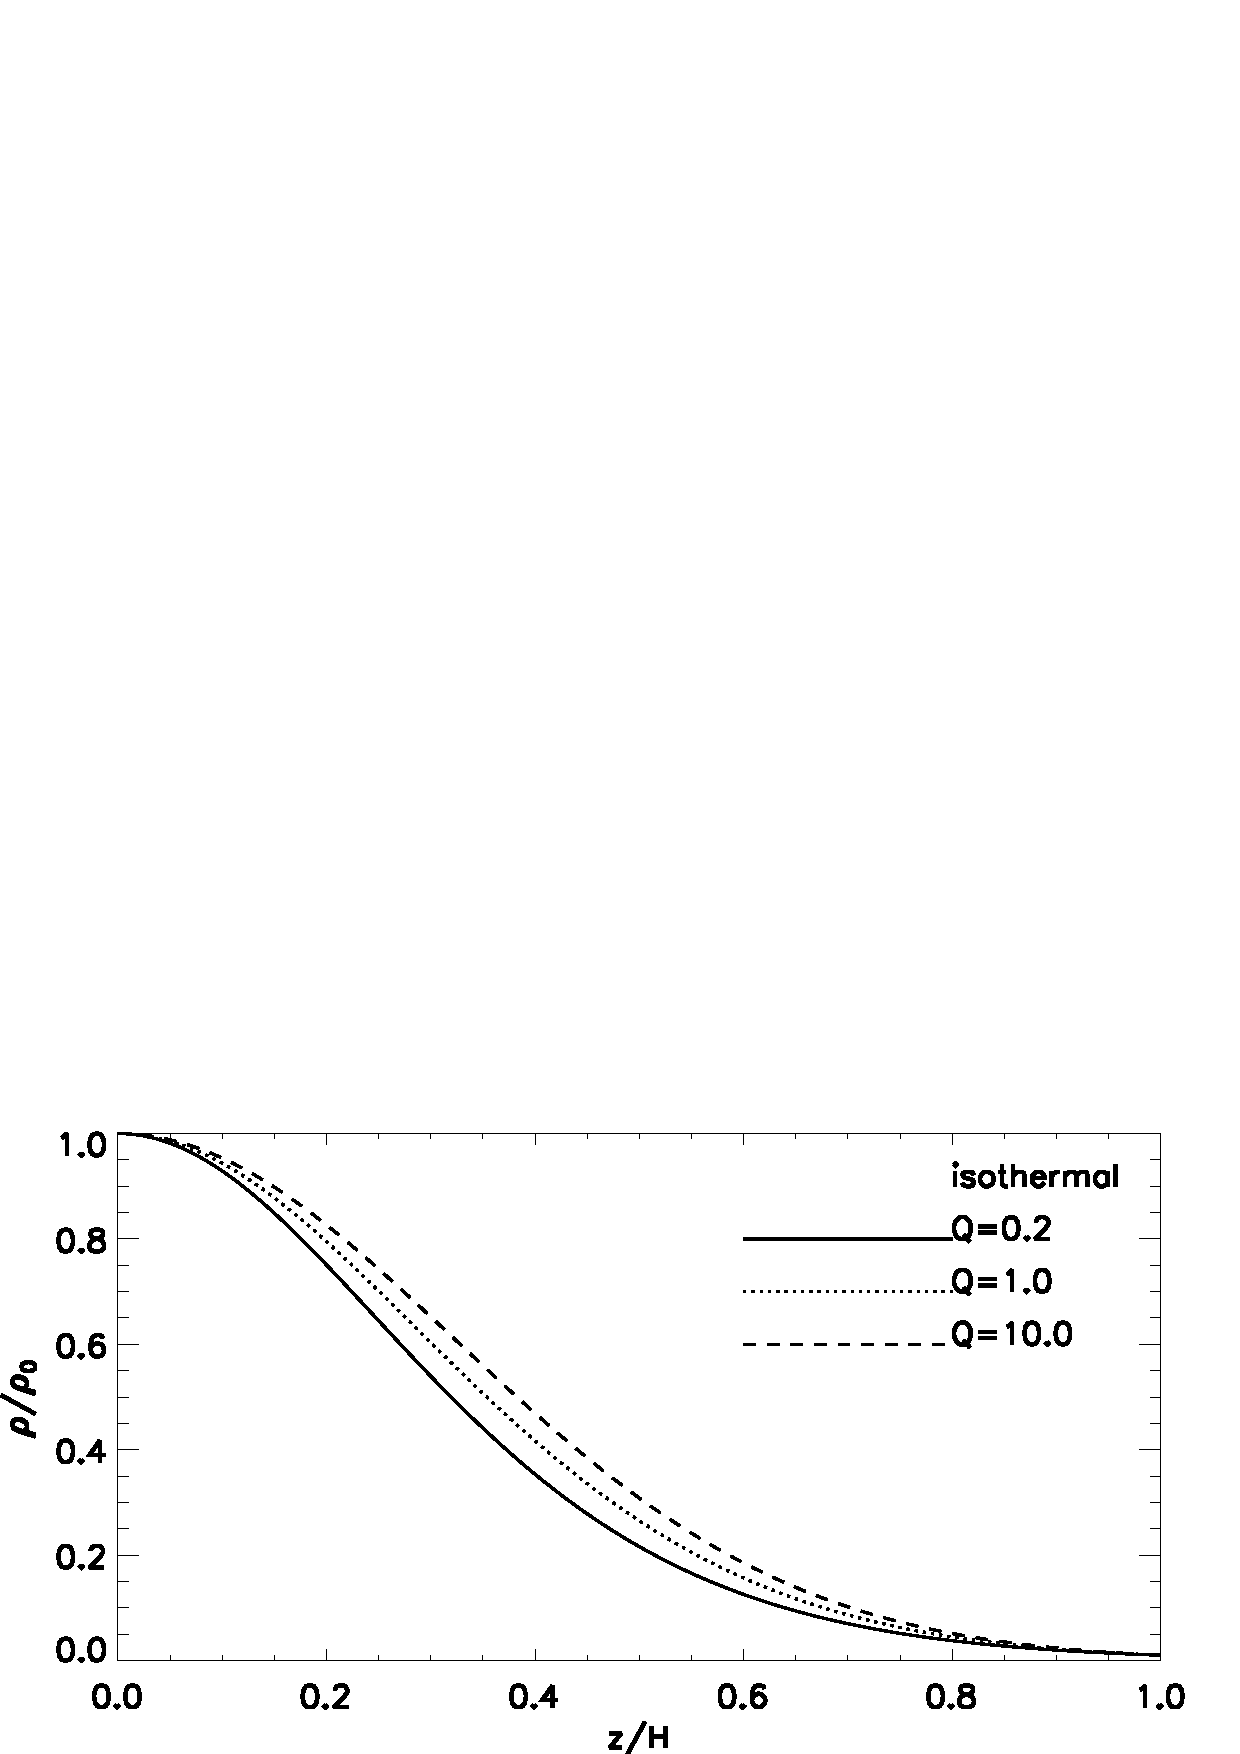
\includegraphics[width=\linewidth,clip=true,trim=0cm 1.5cm 0cm
    0cm]{figures/compare_iso_density} 
  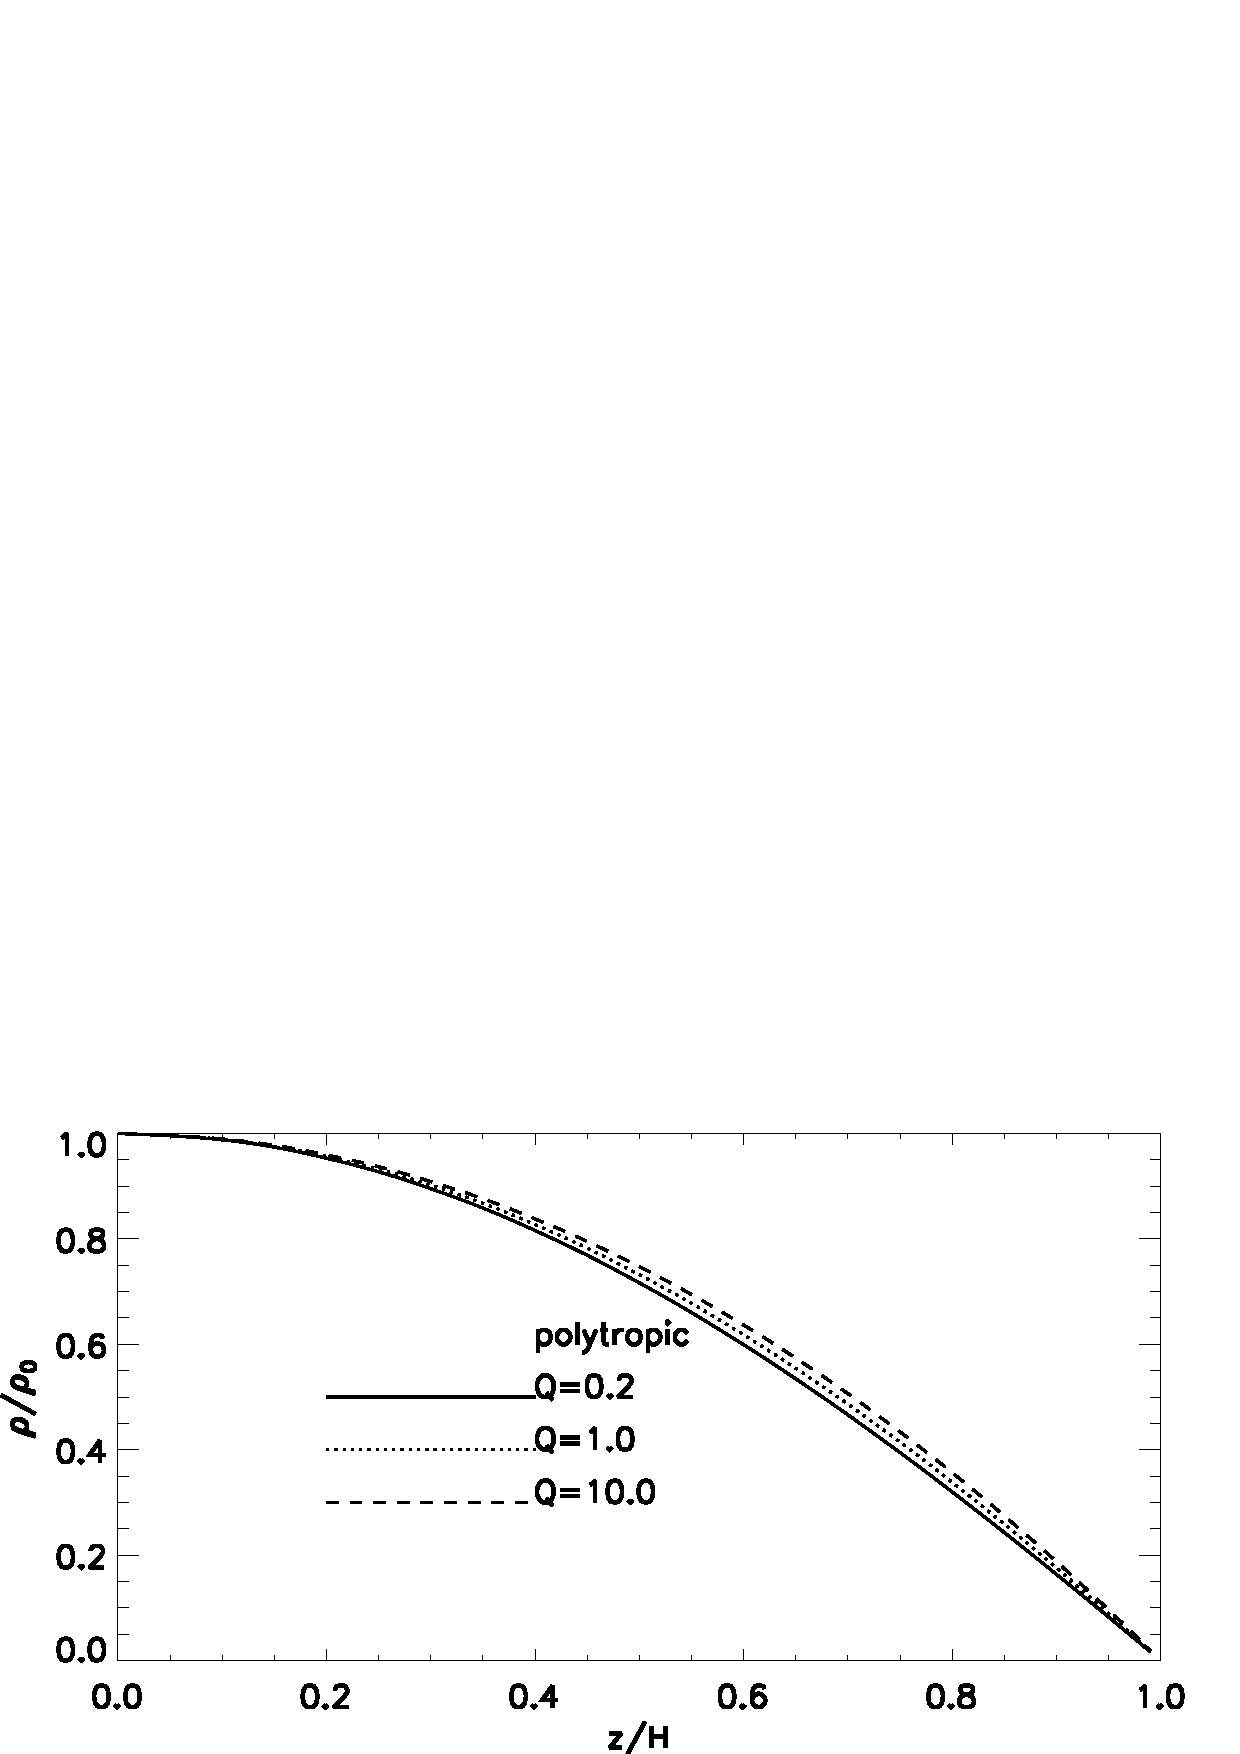
\includegraphics[width=\linewidth,clip=true,trim=0cm 0cm 0cm
    0.9cm]{figures/compare_poly_density} 
  \caption{Equilibrium density field from solving Eq. \ref{eqm_eqns1}
    --- \ref{eqm_eqns2} subject to an isothermal (top) and polytropic
    (bottom) equation of state. Note that the normalization for the
    horizontal axis also depends on the strength of self-gravity,
    i.e. $H=H(Q)$ and is an increasing function of $Q$. 
    \label{eqm_den}}
\end{figure}


\subsection{Resistivity profile}\label{resis_profile}
We adopt constant resistivity or a 
resistivity prescription such that $\eta(z)$ increase {\bf towards} the
midplane. In the latter case, we follow \cite{fleming03} and use 
the resistivity profile 
\begin{align}
  \eta(z) =
  \sqrt{2}\eta_0\left[\exp{\left(-g_+\right)}+\exp{\left(-g_-\right)}\right]^{-1/2},  
\end{align}
where
\begin{align}
  &g_\pm(z) =  \frac{\Sigma_\pm(z)-\Sigma_0}{\Sigma_*}, \\
  &\Sigma_\pm(z) = \int_{\pm z}^\infty\rho(z^\prime)dz^\prime, \label{sigma_pm}
\end{align}
and $\Sigma_0\equiv\Sigma_{\pm}(0)$, so that $g_\pm(0)=0$ and $\eta_0 
= \eta(0)$. The constant $\Sigma_*$ is chosen such that 
\begin{align}
  \cosh{\left(\frac{\Sigma_0}{\Sigma_*}\right)} =
  \left[\frac{\eta_0}{\eta(\infty)}\right]^2,
\end{align}
and we define $\eta_0/\eta(\infty)\equiv A$ as the conductivity 
boost factor from the midplane to the disk surface. We remark that
once $\rho$ and $d\rho/dz$ are obtained from
Eq. \ref{eqm_eqns1} --- \ref{eqm_eqns2}, the integration for
Eq. \ref{sigma_pm} can be performed implicitly by using Poisson's 
equation. 

We use the Elsasser number $\Lambda$ a non-dimensional measure of
conductivity,
\begin{align} 
  \Lambda \equiv \frac{v_A^2}{\eta\Omega},
\end{align}
where $v_A \equiv B_z/\sqrt{\mu_0\rho}$ is the vertical Alfven speed. 
Because of the density stratification, the Elsasser number 
increases with height even for constant resistivity. The disk may be
considered ideal where $\Lambda \gtrsim 1$. 


\subsection{Disk parameters}
%The main parameters describing the resistive, self-gravitating
%shearing box is as follows. 
The strength of self-gravity is
parametrized by 
\begin{align}
  Q \equiv \frac{\Omega^2}{4\pi G\rho_0}
\end{align}
\citep{mamat10}, which is used to set the midplane density $\rho_0$. 
A relation between $Q$ and the Toomre parameter for gravitational
instability of razor-thin disks, $Q_\mathrm{2D}$, is described in
Appendix \ref{q3d2d}.  

The plasma $\beta$ measures the inverse strength of the  
magnetic field 
\begin{align}
  \beta \equiv \frac{\csmid^2}{v_{A0}^2} =
  \frac{\csmid^2\mu_0\rho_0}{B_z^2},  
\end{align}
where $v_{A0}$ is the midplane Alfven speed. Note that we use 
the vertical field for this definition throughout this paper. 

The strength of conductivity is measured by the midplane Elsasser
number   
\begin{align}
  \Lambda_0 \equiv\Lambda(0) =  \frac{v_{A0}^2}{\eta_0\Omega}. 
\end{align}
For non-uniform resistivity we also specify $A > 1$. 

\section{Linear problem}\label{linear}
We consider axisymmetric Eulerian perturbations to the above
equilibrium in the form $\real[\dd\rho(z)\exp{\imgi(k_xx + \sigma
    t)}]$ and similarly for other fluid variables. Here, $k_x$ is a
constant radial wavenumber and $\sigma=-(\omega +\imgi\gamma)$ is a
complex  frequency, where $-\omega$ is the real mode frequency and $\gamma$ is
the growth rate. We take $k_x>0$ without loss of generality. 
Hereafter, we surpress the exponential factor, as
well as the real part notation. 

The linearized continuity equation is 
\begin{align}
  \frac{\imgi\sigma}{c_s^2}W + \imgi k_x \dd v_x
  +\left(\ln\rho\right)^\prime\dd v_z + \dd v_z^\prime = 0,\label{lin_cont}
\end{align}
where $^\prime$ denotes $d/dz$ and $W=\delta P/\rho =
c_s^2\delta\rho/\rho$ is the enthalpy perturbation.  
The linearized equations of motion are
\begin{align}
  &\imgi\sigma \dvx - 2\Omega\dvy  = - \imgi
  k_x\w + \frac{B_z}{\mu_0\rho} \left[\dbx^\prime - \imgi 
    k_x\left(\dbz + \epsilon\dby\right)\right],\\
  &\imgi\sigma\dvy + 
    \frac{\kappa^2}{2\Omega}\dvx = \frac{B_z}{\mu_0\rho}\dby^\prime\label{lin_vy},\\ 
  & \imgi\sigma\dvz = -\w^\prime - \frac{B_y}{\mu_0\rho}\dby^\prime\label{lin_vz},  
\end{align}
where the effective enthalpy perturbation
$\w = W + \dphi$. The linearized induction equation is
\begin{align}
&  \imgi\bar{\sigma}\dbx = B_z\dvx^\prime +
  \eta\dbx^{\prime\prime}+\eta^\prime\dbx^\prime - \imgi k_x
  \eta^\prime \dbz,\label{induct_x}\\
&\imgi\bar{\sigma}\dby = B_z\dvy^\prime -B_y\Delta - S\dbx +
  \eta\dby^{\prime\prime}+\eta^\prime\dby^\prime,\label{induct_y}\\
& \imgi\bar{\sigma}\dbz = -\imgi  k_xB_z \dvx +
\eta\dbz^{\prime\prime}, \label{induct_vert}
%& \imgi\bar{\sigma}\dbz = -\imgi  k_x \dvx  -\imgi k_x\eta \dbx^{\prime}, \label{induct_vert}
\end{align} 
where $\imgi\bar{\sigma} = \imgi\sigma + \eta k_x^2$,
$\Delta\equiv \nabla\cdot\bm{\delta v}  = \imgi k_x\dvx + \dvz^\prime$,   
and the divergence-free condition is $\imgi k_x\dbx +
\dbz^\prime=0$. Finally, the linearized Poisson equation is 
\begin{align}
  \dphi^{\prime\prime} - k_x^2\dphi = \frac{\Omega^2\rho}{c_s^2Q\rho_0}W.  \label{lin_poisson}
\end{align}

We eliminate $\dd\bm{B}$ and $\dvz$ between the linearized
equations to obtain a system of ordinary differential equations for
$\bm{U}=\left(\dvx,\dvy,W,\dphi\right)$. We detail the steps 
in Appendix \ref{reduction} for two cases considered in this paper:
%We consider two cases:
\begin{enumerate}
\item Purely vertical field with constant or variable
  resistivity (see below), so that $\epsilon = 0$ and $\eta=\eta(z)$. 
\item Tilted field with uniform resistivity
  so that $\epsilon \neq 0$ and $\eta=\rm{constant}$.   
\end{enumerate}
Schematically, the numerical problem is to solve 
\begin{align}
  L_{11}\dvx + L_{12}\dvy + L_{13}W + L_{14}\dphi &= 0, \label{lin1}\\
  L_{21}\dvx + L_{22}\dvy + L_{23}W + L_{24}\dphi &= 0, \label{lin2}\\
  L_{31}\dvx +L_{32}\dvy + L_{33}W + L_{34}\dphi &=0,\label{lin3}\\
  \phantom{L_{31}\dvx + L_{22}\dvy +} L_{43}W + L_{44}\dphi
  &=0\label{lin4},
\end{align}
where differential operators $L_{1j},\,L_{2j}$ and $L_{3j}$
($j=1,2,3,4$) can be read off Appendix \ref{reduction} and $L_{4j}$
($j=3,4$) from the linearized Poisson equation above. We remark that
the more general problem of tilted field and variable resistivity
%($\epsilon\neq0$ and $\eta=\eta(z)$
can also be reduced to the above form. 


%where the differential operators $L_{1j}$, $L_{2j}$ and $L_{3j}$ can
%be read off Eq. \ref{final_vx}, Eq. \ref{final_vy} and 
%Eq. \ref{final_w} respectively, and $L_{4j}$ from
%Eq. \ref{lin_poisson}. 

%Note that $L_{13},\,L_{14},\,L_{23},\,L_{24}$ and $L_{31}$ are
%proportional to $k_x$. Then for for $k_x=0$ 
%Eq. \ref{lin1}---\ref{lin2} are decoupled from 
%Eq. \ref{lin3}---\ref{lin4}. In this case, a solution is $\dphi=W=0$,
%with $\dvx$ and $\dvy$ determined by $L_{11}\dvx + L_{12}\dvy = 0$ and 
%$L_{21}\dvx + L_{22}\dvy=0$, which is the incompressible MRI problem. 
%This means that the density and potential perturbations can only
%influence the MRI for $k_x\neq0$. Nevertheless, for $k_x=0$,
%self-gravity can still have an effect through the background
%equilibrium.  


\subsection{Domain and boundary conditions}

\subsubsection{Case 1: vertical field}
We impose $\bm{U}$ to be an even function of $z$, so that
$d\bm{U}/dz=0$ at $z=0$. This reduces the computational domain to
$z\in[0,Z_s]$ and permits higher numerical resolution. At the disk
surface we set %$\dbx=\dby=\dvz=0$ 
\begin{align}
  \dbx(Z_s) = \dby(Z_s) = \dvz (Z_s) = 0, 
\end{align}
so the field remains vertical. The potential boundary
condition is 
\begin{align}
  \dphi^\prime(\zmax) + k_x\dphi(\zmax) = 0 \label{pot_bc1}
\end{align}
\citep{goldreich65a}. 

\subsubsection{Case 2: tilted field} 
In this more general setup the computational domain is
$z\in[-Z_s, Z_s]$. At the disk surfaces we adopt the `halo' model of
\cite{gammie94}, so that
\begin{align}
  \Delta(\pm Z_s) & = 0, \\
  \dby(\pm Z_s) & = 0,\\
  \dbz(\pm Z_s) \mp \imgi \dbx(\pm Z_s) &= 0,
\end{align}
and the potential boundary condition is 
\begin{align}
  \dphi^\prime(\pm \zmax) \pm k_x\dphi(\pm\zmax) =  - \left. \frac{\Omega^2
    \rho \xi_z}{\rho_0Q}\right|_{\pm\zmax}, \label{pot_bc2}
\end{align}
where $\xi_z=\dvz/\imgi\sigma$ is the vertical Lagrangian
displacement. In practice,  Eq. \ref{pot_bc1} and \ref{pot_bc2} are
very similar because $\rho(\pm\zmax)\ll\rho_0$. 

%We adopt two kinds of vertical boundary conditions depending on the
%field geometry. 
%In both case 1 and case 2 the potential boundary
%condition is 
%\begin{align}
%  \dphi^\prime(\zmax) \pm k_x\dphi(\zmax) = 0
%\end{align}

%At the vertical disk boundaries $z=\pm\zmax$ we assume  
%$\dvz=\dbx=\dby=0$, and 

%for the potential perturbation \citep[see][]{goldreich65a}, where the
%upper (lower) sign applies to the upper (lower) disk surface. 
%For Case 1 (purely vertical field) we additionally assume $\bm{U}$ is
%an even function of $z$, so that $d\bm{U}/dz=0$ 
%at $z=0$. 

%This implies that $\dbx=\dby=0$ at the midplane, consistent
%with a highly resistive dead zone. 

\subsection{Numerical procedure}
We use a pseudo-spectral method to solve the set of linearized
equations. Let
\begin{align}\label{cheby_expand}
  \bm{U}(z) 
  = \sum_{k=1}^{N_z} \bm{U}_k\psi_k(z/\zmax), 
\end{align}
where 
\begin{align}
  \psi_k  = 
  \begin{cases}
    T_{2(k-1)} & B_y \equiv 0 \text{ (case 1)},\\
    T_{k-1}   & B_y\neq 0 \text{ (case 2)},
  \end{cases}
\end{align}
and  $T_l$ is a Chebyshev polynomial of the first kind of order $l$
\citep{stegun65}. Note that for case 1 the midplane symmetry condition
is taken care of by the choice of basis functions. 
%Note that in case 1
%The number of basis functions is
%$N_z$ and $l_\mathrm{max}=2(N_Z-1)$ is the highest polynomial order. 
%For a vertical field we only use even Chebyshev polynomials 
%to satisfy the symmetry condition at $z=0$, so in case 1 we only
%consider $z\geq 0$.  

The pseudo-spectral coefficients $\bm{U}_n$  are obtained by demanding
the set of linear equations to be satisfied at $N_z$ collocation
points along the vertical direction. We choose these points as the
extrema of $T_{l_\mathrm{max}}$ plus end points, where
$l_\mathrm{max}$ is the highest polynomial order. Our standard
resolution is $N_z=256$.  

The above procedure discretizes the linear equations to a matrix equation,
\begin{align}\label{matrix_eqn}
\bm{M}\bm{w} = 0, 
\end{align}
where $\bm{M}$ is a $4N_z\times 4 N_z$ matrix representing the $L_{ij}$ 
and upper disk boundary conditions, 
and $\bm{w}$ is a vector storing the pseudo-spectral coefficients. 
Starting with an initial guess for $\sigma$, non-trivial solutions to
Eq. \ref{matrix_eqn} are obtained by varying $\sigma$ using Newton-Raphson iteration 
such that $\mathrm{det}\bm{M}=0$ \citep[details can be found in][]{lin12}.


\subsubsection{Non-dimensionalization}\label{non-dim}
We solve the linearized equations in non-dimensional form,
by defining
%We further write 
\begin{align}
  &z=\hat{z}H,\quad k_x =  \hat{k}_x/H,\quad \sigma = \hat{\sigma}\Omega,
  \quad \delta\bm{v} = \csmid 
  \delta\hat{\bm{v}}, \\ 
  &\delta\bm{B} = B_z\delta\hat{\bm{B}},\quad
  \delta\rho = \rho\hat{W}/\hat{c}_s^2,\quad \delta\Phi =
  \csmid^2\delta\hat{\Phi},  
\end{align} 
where $\hat{c}_s=c_s/\csmid$. We also non-dimensionalize other
background quantities, i.e. $\hat{v}_A=v_A/\csmid$,
$\hat{S}=S/\Omega$, $\hat{\kappa}=\kappa/\Omega$,
$\hat{\Omega}_z=\Omega_z/\Omega$ and $\hat{\eta} = \eta/(H^2\Omega)$. 


\subsection{Diagnostics}
We visualize results in terms of dimensionless energy densities. We
define 
\begin{align}
  &E_m \equiv \frac{|\delta \hat{\bm{B}}|^2}{2\beta},\\
  &E_g =
  \frac{\hat{\rho}}{\hat{c}_s^2}\left|\real\left(\hat{W}\dd\hat{\Phi}^*\right)\right|,\\  
  &E_k = \frac{1}{2}\hat{\rho}|\delta\hat{\bm{v}}|^2,\\
  &E_t = \frac{\hat{\rho}|\hat{W}|^2}{2\hat{c}_s^2},
\end{align}
as the perturbed magnetic, gravitational, kinetic and thermal
energies, respectively, which are functions of $z$. The total energy
is $E=E_m+E_g+E_k+E_t$. We use $\avg{\cdot}$ to denote an average over
$z$. 
%and we then normalize $E_i$ by
%$\mathrm{max}(E)$.  
 

\section{MRI in self-gravitating disks}\label{result1}
In this section we focus on the MRI and use the vertical field setup
of case 1. We first consider MRI modes with negligible density/potential
perturbations to see the effect of self-gravity on the MRI through the
background stratification, then go on to examine MRI modes with
density/potential perturbations in massive disks.  

\subsection{Influence of self-gravity on the MRI through the
  background equilibrium}
Here we use polytropic disks, which have a well-defined disk
thickness. The upper disk boundary is set to $Z_s=0.99H$. We fix
$\beta=100$ and $k_xH=0.1$ unless otherwise stated. 

\subsubsection{Uniform
  resistivity}   
Fig. \ref{compare_growth_poly_uniresis} plots MRI growth rates as a
function of $Q$ and $\Lambda_0$. The resistivity is uniform ($A=1$). 
For ideal MHD ($\Lambda_0>1$), there is negligible dependence on
$Q$. In the resistive limit   
($\Lambda_0<1$), however, growth rates decrease noticeably for $Q<0.5$
($Q_\mathrm{2D}\lesssim 1.5$).  Since we find density and potential
perturbations to be negligible (i.e. the linear response is
non-self-gravitating), this shows that disk self-gravity can affect the
MRI through the background equilibrium.

\begin{figure}
  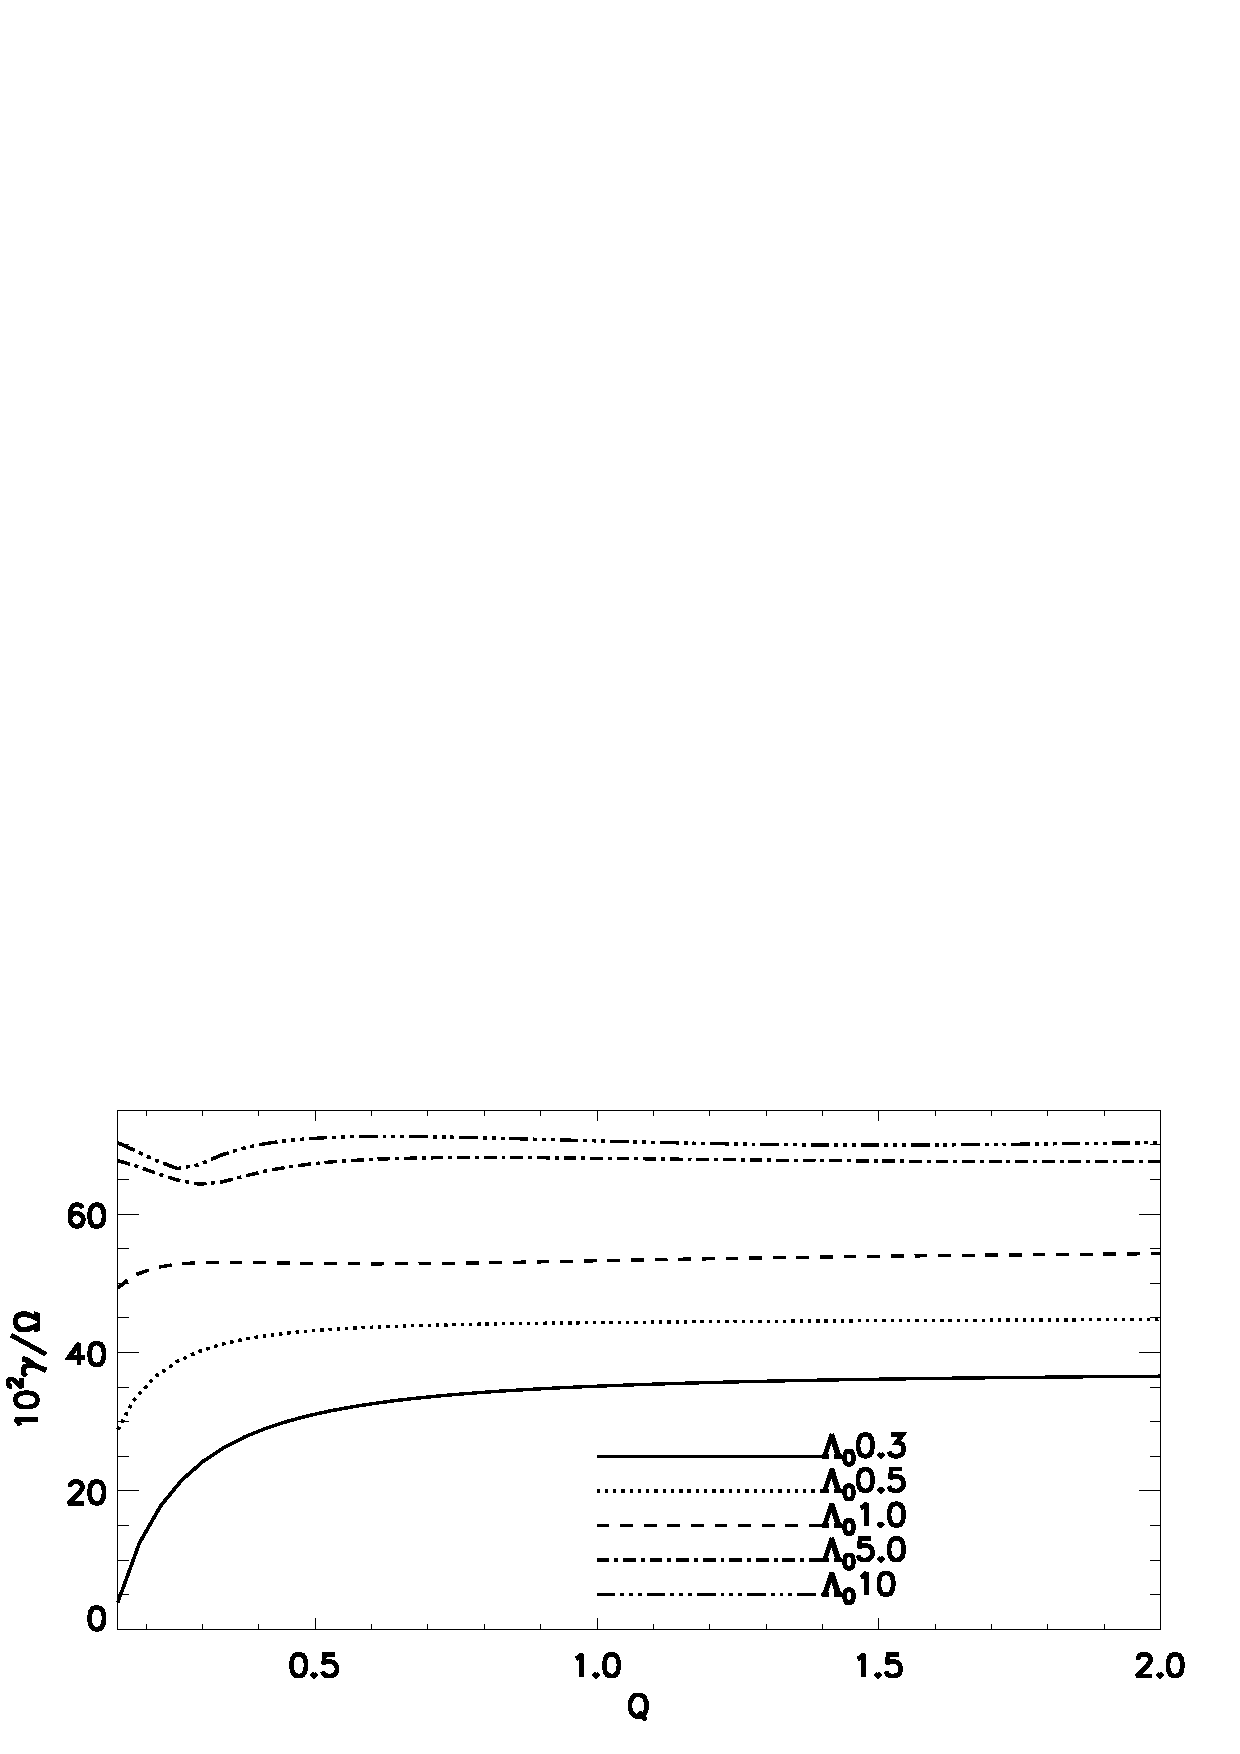
\includegraphics[width=\linewidth]{figures/compare_growth_poly_uniresis2}
  \caption{MRI growth rates as a function of $Q$ and midplane 
    Elsasser numbers, in polytropic disks with $\beta=100$ and uniform
    resistivity.  
    \label{compare_growth_poly_uniresis}}
\end{figure}

\cite{sano99} found that for MRI to operate, its 
wavelength $\lambda$ should fit inside the disk. That is,   
\begin{align}\label{sano_crit}
  \lambda \equiv
  \mathrm{max}\left(\lambda_\mathrm{ideal},\lambda_\mathrm{resis}\right)\lesssim
  2H, 
\end{align}
where the MRI wavelengths are given by 
\begin{align}\label{lambda_ideal}
  \frac{\lambda_\mathrm{ideal}}{2H} = \frac{4\pi}{\sqrt{15}} f \hat{v}_A =
  \frac{4\pi f}{\sqrt{15\beta\hat{\rho}}}
\end{align}
for ideal MHD, and 
\begin{align}\label{lambda_resis}
  \frac{\lambda_\mathrm{resis}}{2H} = \frac{2\pi}{\sqrt{3}}\frac{\hat{\eta}}{\hat{v}_A f} =
  \frac{2\pi f}{\Lambda_0}\sqrt{\frac{\hat{\rho}}{3\beta}} 
\end{align}
in the limit of high resistivity.  
   
Because $\hat{\rho}$ is weakly dependent
on $Q$ (Fig. \ref{eqm_den}), self-gravity only affects the
MRI through the factor $f$, which increases with decreasing $Q$ (see
Fig. \ref{plot_fq} in Appendix \ref{appen1}).   
This implies that sufficiently strong self-gravity can stabilize the
MRI by making $ 2H<\lambda $.   
 
In the ideal limit, we find $\lambda < 2H$ throughout most of the disk
for the values of $Q$ considered, so self-gravity does not affect
growth rates significantly. However, the ratio $\lambda/2H$ does
increase with stronger self-gravity. Consequently, the wavelength of
the instability, in units of $H$, increases. This is shown in
Fig. \ref{compare_result_lambda10} which plots the magnetic energies
for $\Lambda_0=10$ and a range of $Q$ values. The number of vertical
nodes decrease with $Q$, i.e. the disk accommodates fewer wavelengths
because increasing vertical self-gravity makes it thinner. 

\begin{figure}
  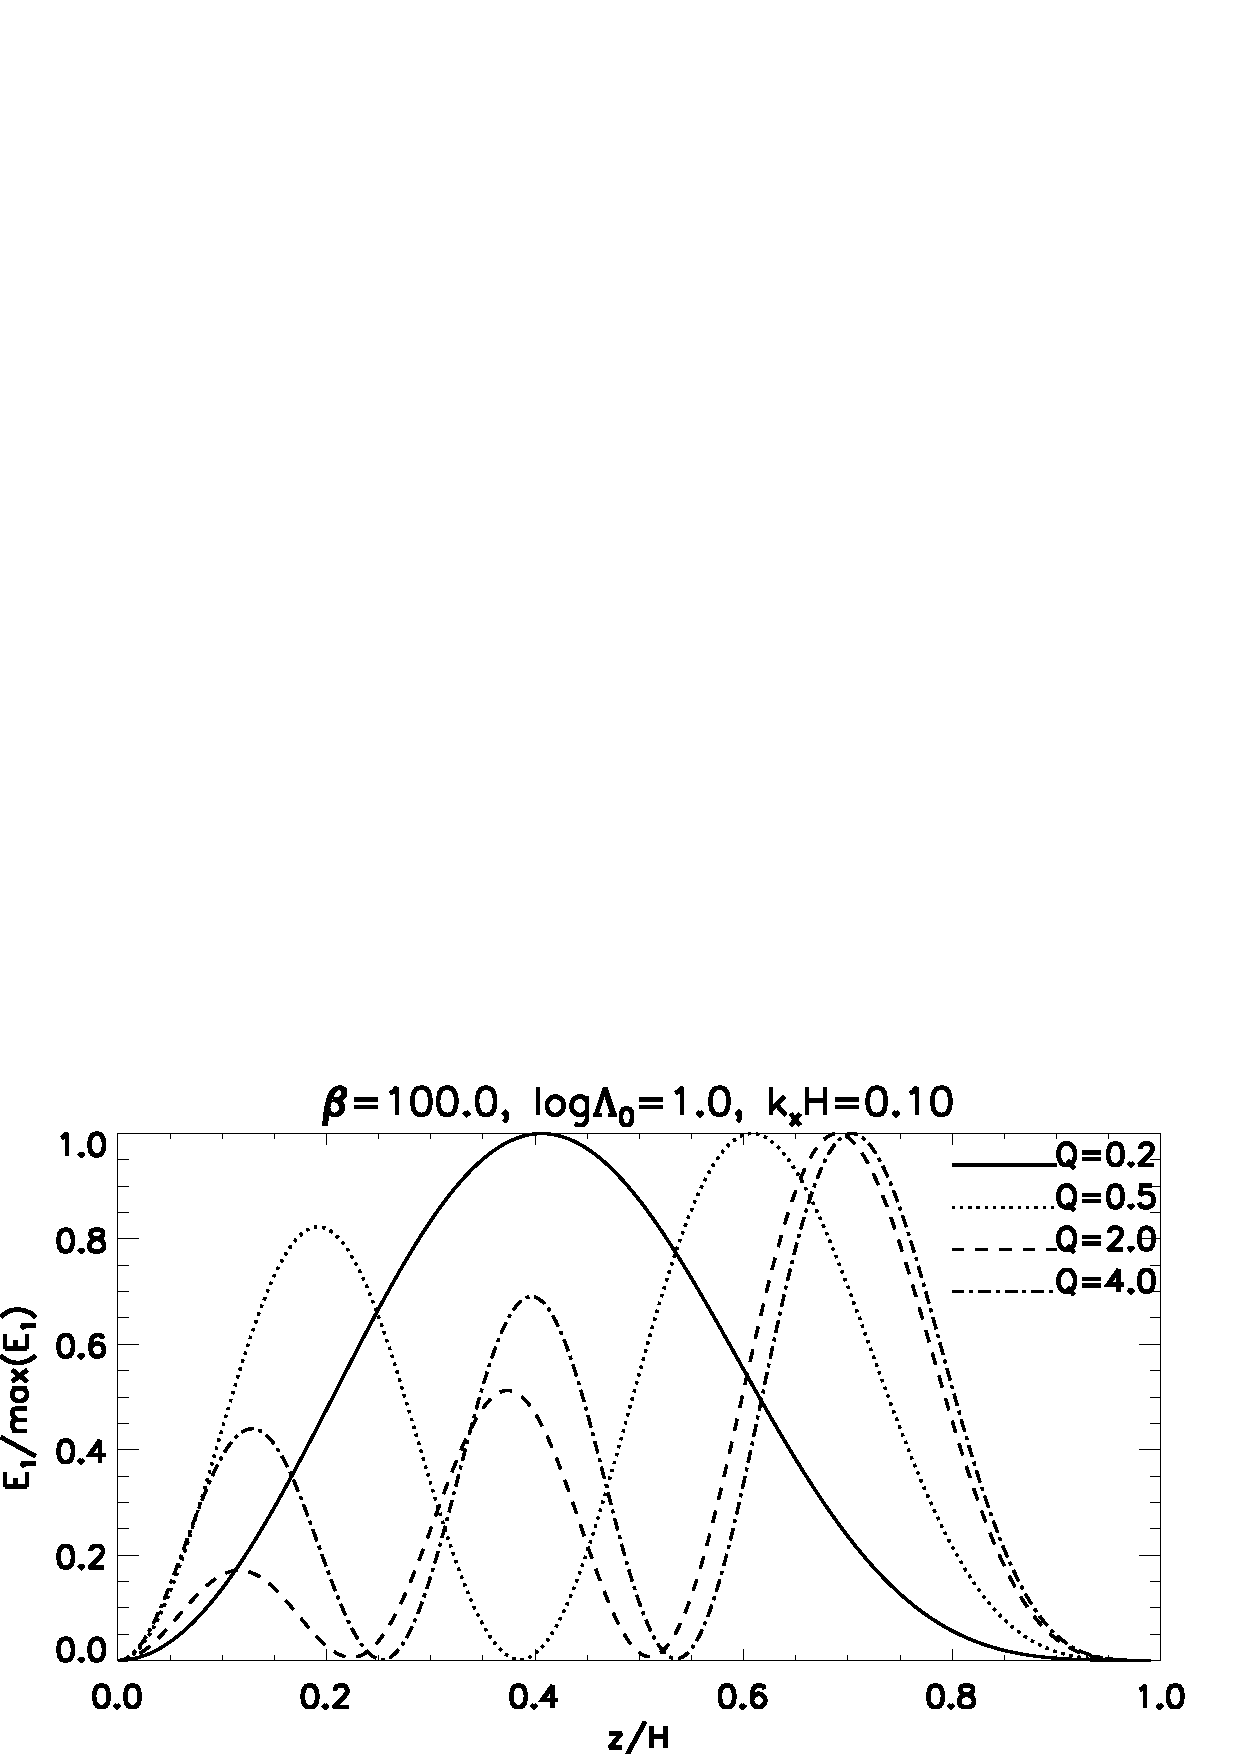
\includegraphics[width=\linewidth]{figures/compare_result_lambda10}
  \caption{MRI magnetic energies in ideal polytropic disks
    for different strengths of self-gravity.    
    \label{compare_result_lambda10}}
\end{figure}


Self-gravity appreciably decreases the MRI growth rates in the
resistive limit. Fig. \ref{lambda_poly_resis} plots 
Eq. \ref{sano_crit} for $\Lambda_0=0.3$. In the non-self-gravitating
disk ($Q=4$) the instability criterion is marginally satisfied and the
MRI operates. As $Q$ decreases, 
Eq. \ref{sano_crit} is violated and the MRI growth rate is
significantly reduced. This is seen for $Q=0.2$ where $\lambda \geq 2H$ throughout
the disk. (The instability is not suppressed since
Eq. \ref{lambda_ideal}---\ref{lambda_resis} is only exact for
unstratified disks.) Although the function 
$f(Q)$ does not change significantly for the range of $Q$ considered,
the dependence of $\lambda_\mathrm{resis}$ on $f(Q)$ is amplified by the
denominator $\Lambda_0<1$ in the resistive case. Modes in
Fig. \ref{lambda_poly_resis} have no nodes in the magnetic energy
$E_m$ except at $z\simeq0,\,H$, i.e. only the longest wavelength survives
with large resistivity. 
%self-gravity tips it over    

\begin{figure}
  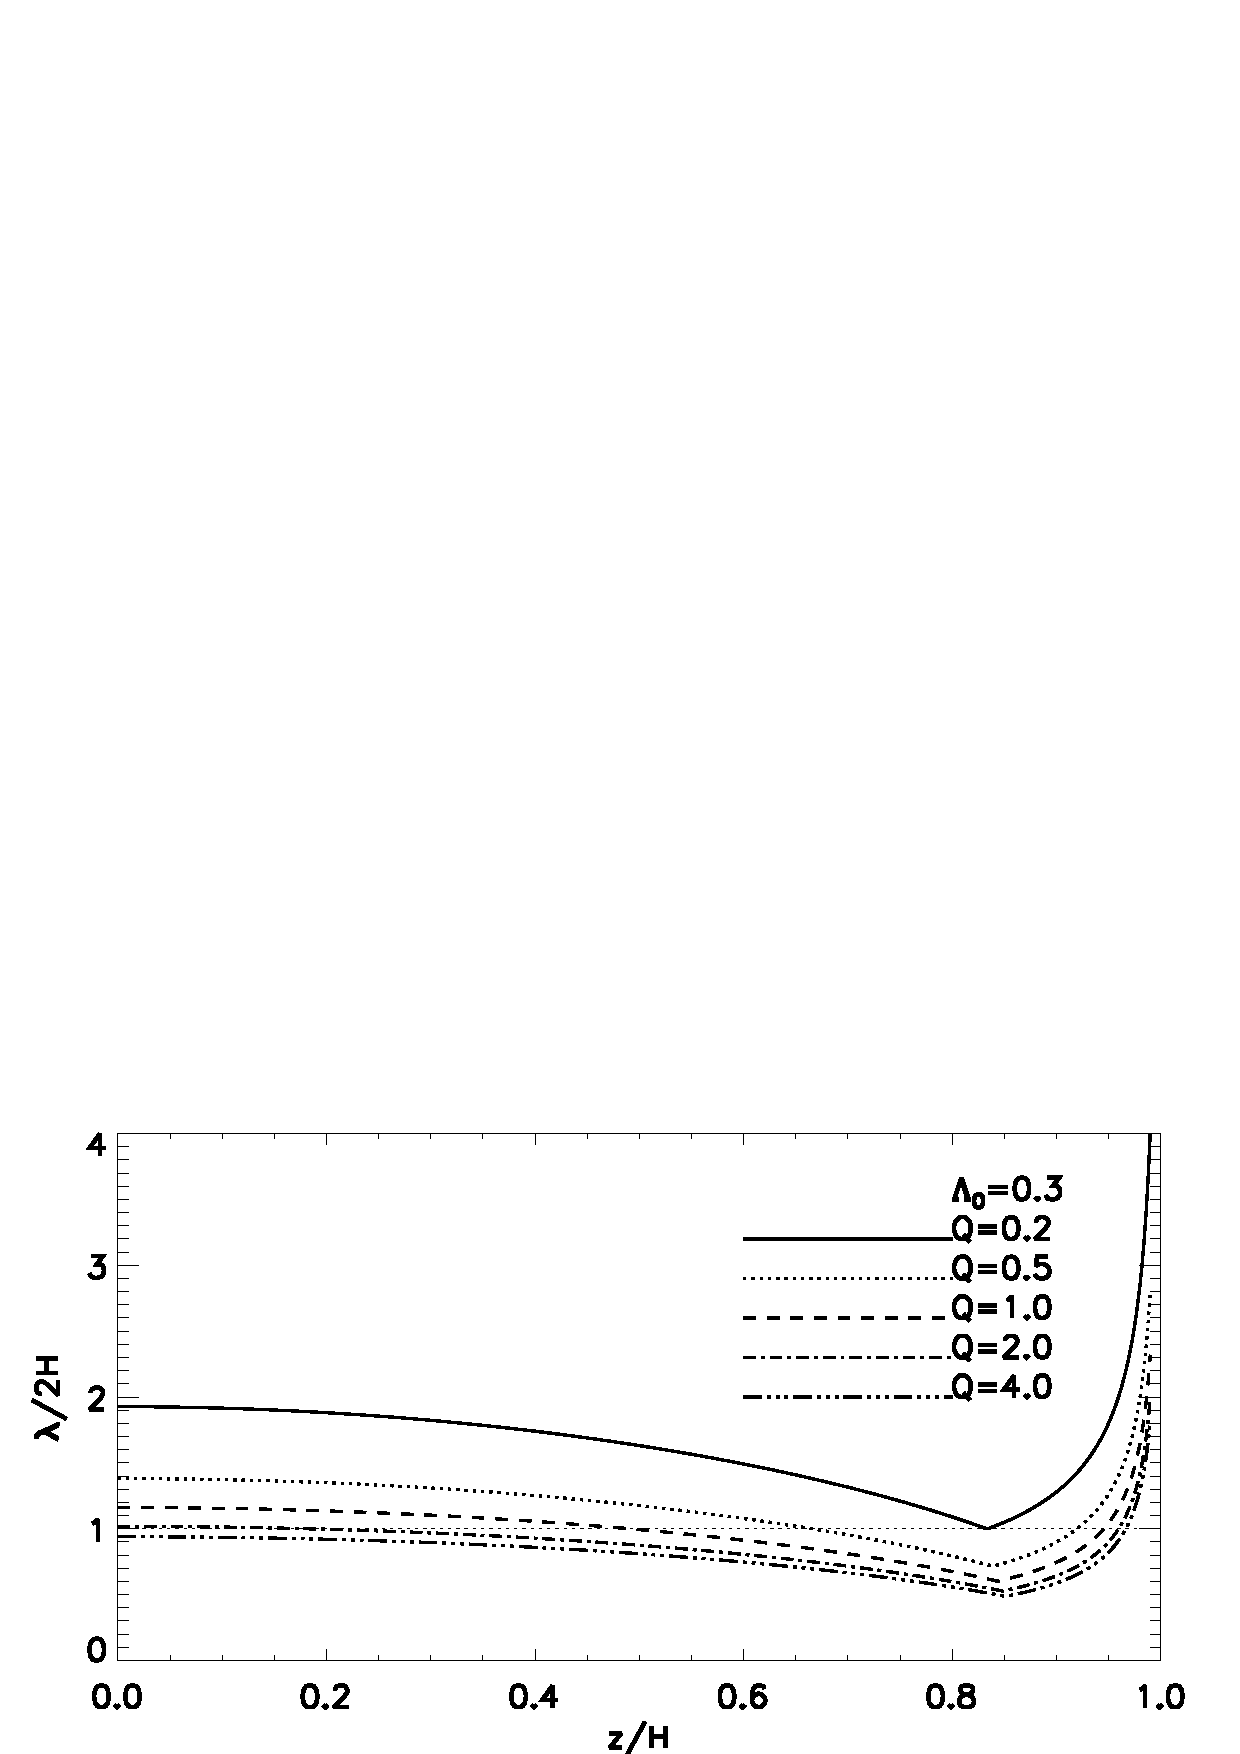
\includegraphics[width=\linewidth]{figures/lambda_poly_uniresis}
  \caption{Approximate wavelengths of the most unstable MRI modes as given by
    Eq. \ref{sano_crit}---\ref{lambda_resis}, normalized by the 
    disk thickness, as a function of height. MRI is expected to
    operate if $\lambda/2H\lesssim 1$. 
    \label{lambda_poly_resis}}
\end{figure}



\subsubsection{Layered 
  resistivity} 
Here we consider disks with midplane Elsasser number $\Lambda_0=0.1$
and a variable resistivity profile with
$A=10^2$. Fig. \ref{poly_layer} compares the magnetic  
energies for $Q=0.2,\,1$ and $4$. They have similar growth rates, $\gamma/\Omega
= 0.53,\,0.64$ and $0.66$, respectively. In the non-self-gravitating
limit ($Q=4$), the MRI is effectively suppressed for
$z\lesssim0.5H$. This is consistent with the picture of layered
accretion proposed for non-self-gravitating disks \citep{gammie96,fleming03}. 
However,in the massive disk ($Q=0.2$) the mode occupies a wider vertical
extent because its wavelength (in units of $H$) is larger. This
suggests that in massive disks, the MRI is not well localized to a
sub-layer within the height, even when the resistivity has a layered
structure.  


\begin{figure}
  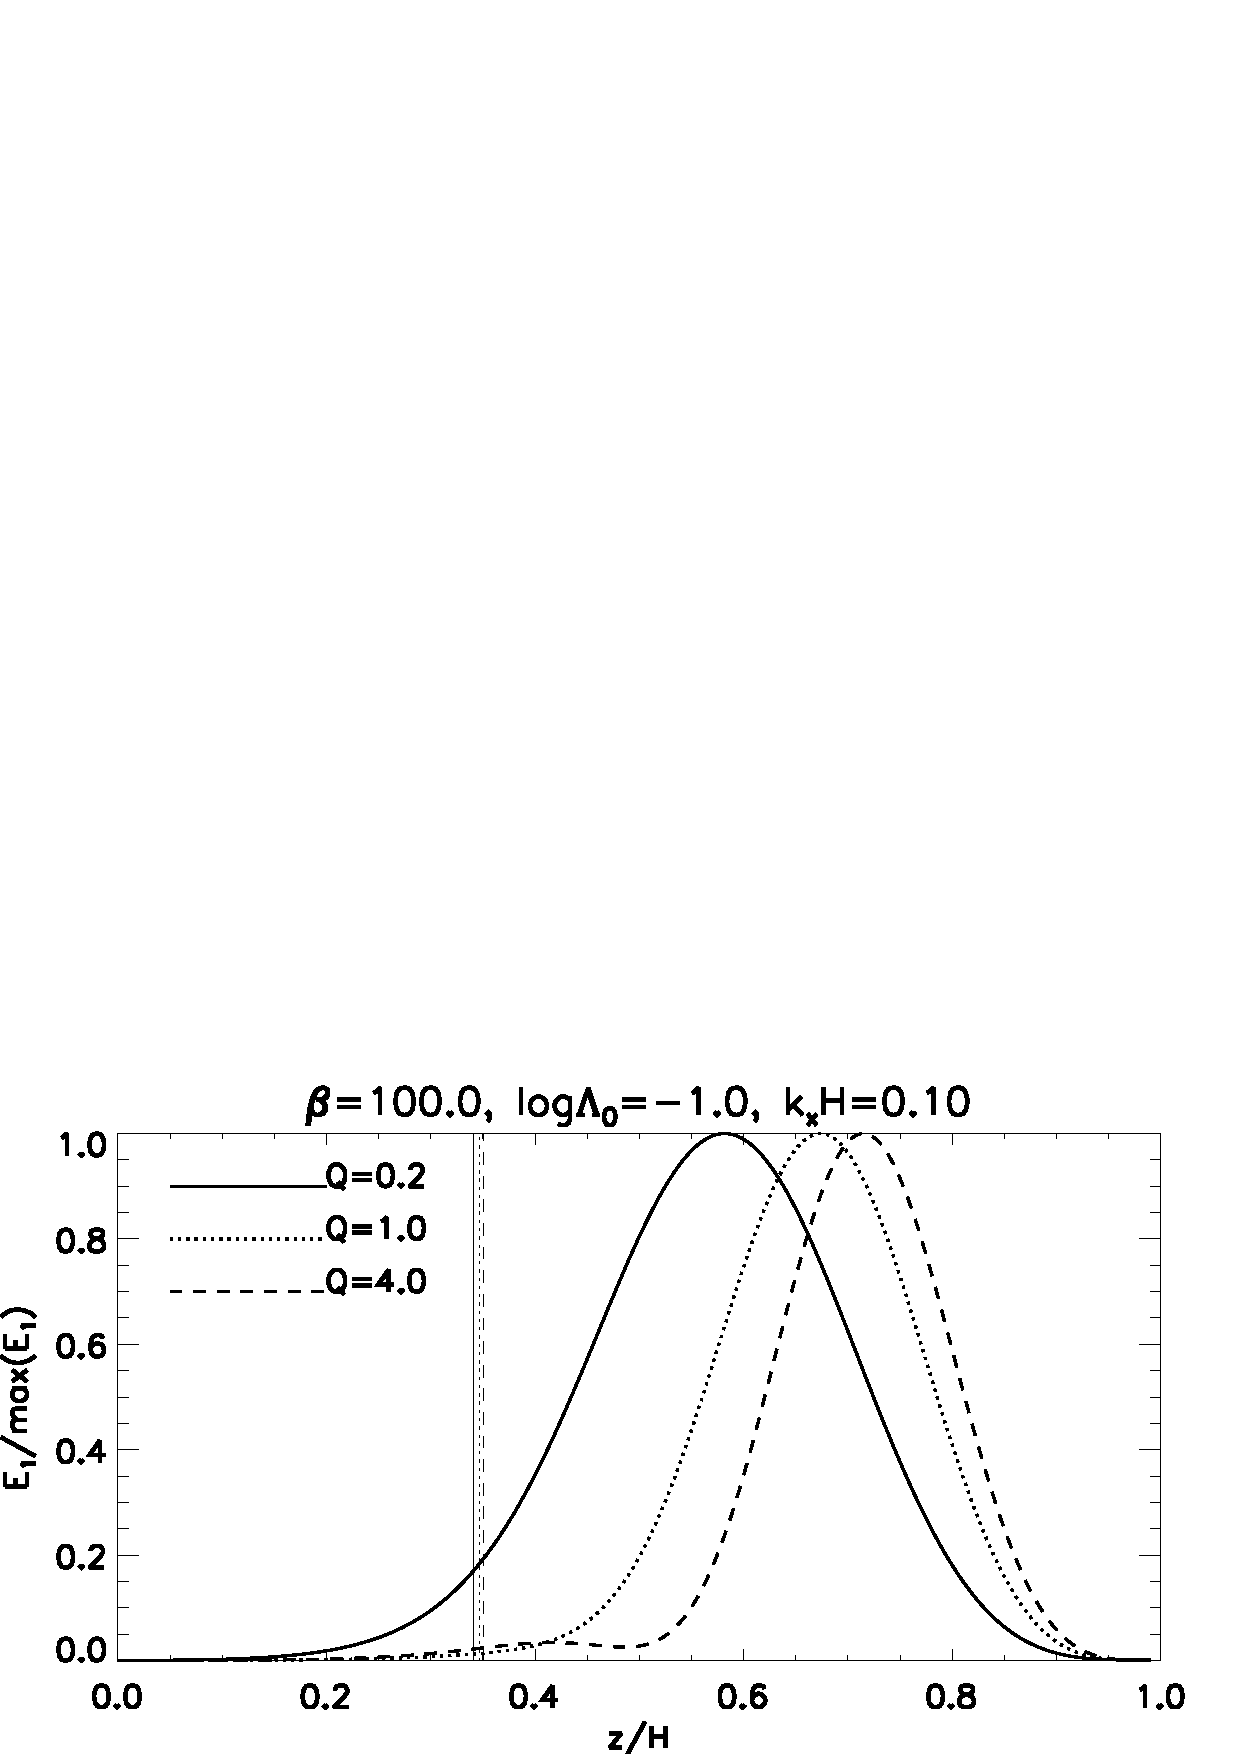
\includegraphics[width=\linewidth]{figures/compare_results_poly_layer_amp100}
  \caption{Magnetic energies as a function of height, for polytropic disks
    in which the conductivity increases by a
    factor $A=10^2$ in going from the midplane to the upper disk
    boundary. The vertical lines indicate $\Lambda=1$ for each value 
    of $Q$.
    \label{poly_layer}}
\end{figure}

\subsubsection{Dependence on $k_x$}
The above experiments show that with increasing 
disk self-gravity, the MRI becomes more global in the vertical
direction. We find a similar result in the horizontal direction. 
Fig. \ref{compare_growth_poly_kx} show MRI growth rates as a
function of $k_x$ for a range of $Q$ values. Increasing self-gravity
decreases the cut-off radial wavenumber for the MRI. We checked
that these modes have negligible density perturbations. Then we can 
understand this result by invoking the instability criteria for  
incompressible MRI in an unstratified Keplerian disk,
\begin{align}
  v_A^2(k_z^2 + k_x^2) < 3\Omega^2,
\end{align}
where $k_z$ is a vertical wavenumber \citep{kim00}. Setting $k_z^2\sim
\Omega^2/v_A^2$ and non-dimensionalizing, we find
\begin{align} 
  k_xH \lesssim \frac{\sqrt{\beta}}{f},
\end{align}
where order-unity factors have been dropped. Despite a simplistic
approach, this demonstrates that with increasing self-gravity
(increasing $f$), we expect MRI modes with small radial
length scales to be suppressed.   


 
\begin{figure}
  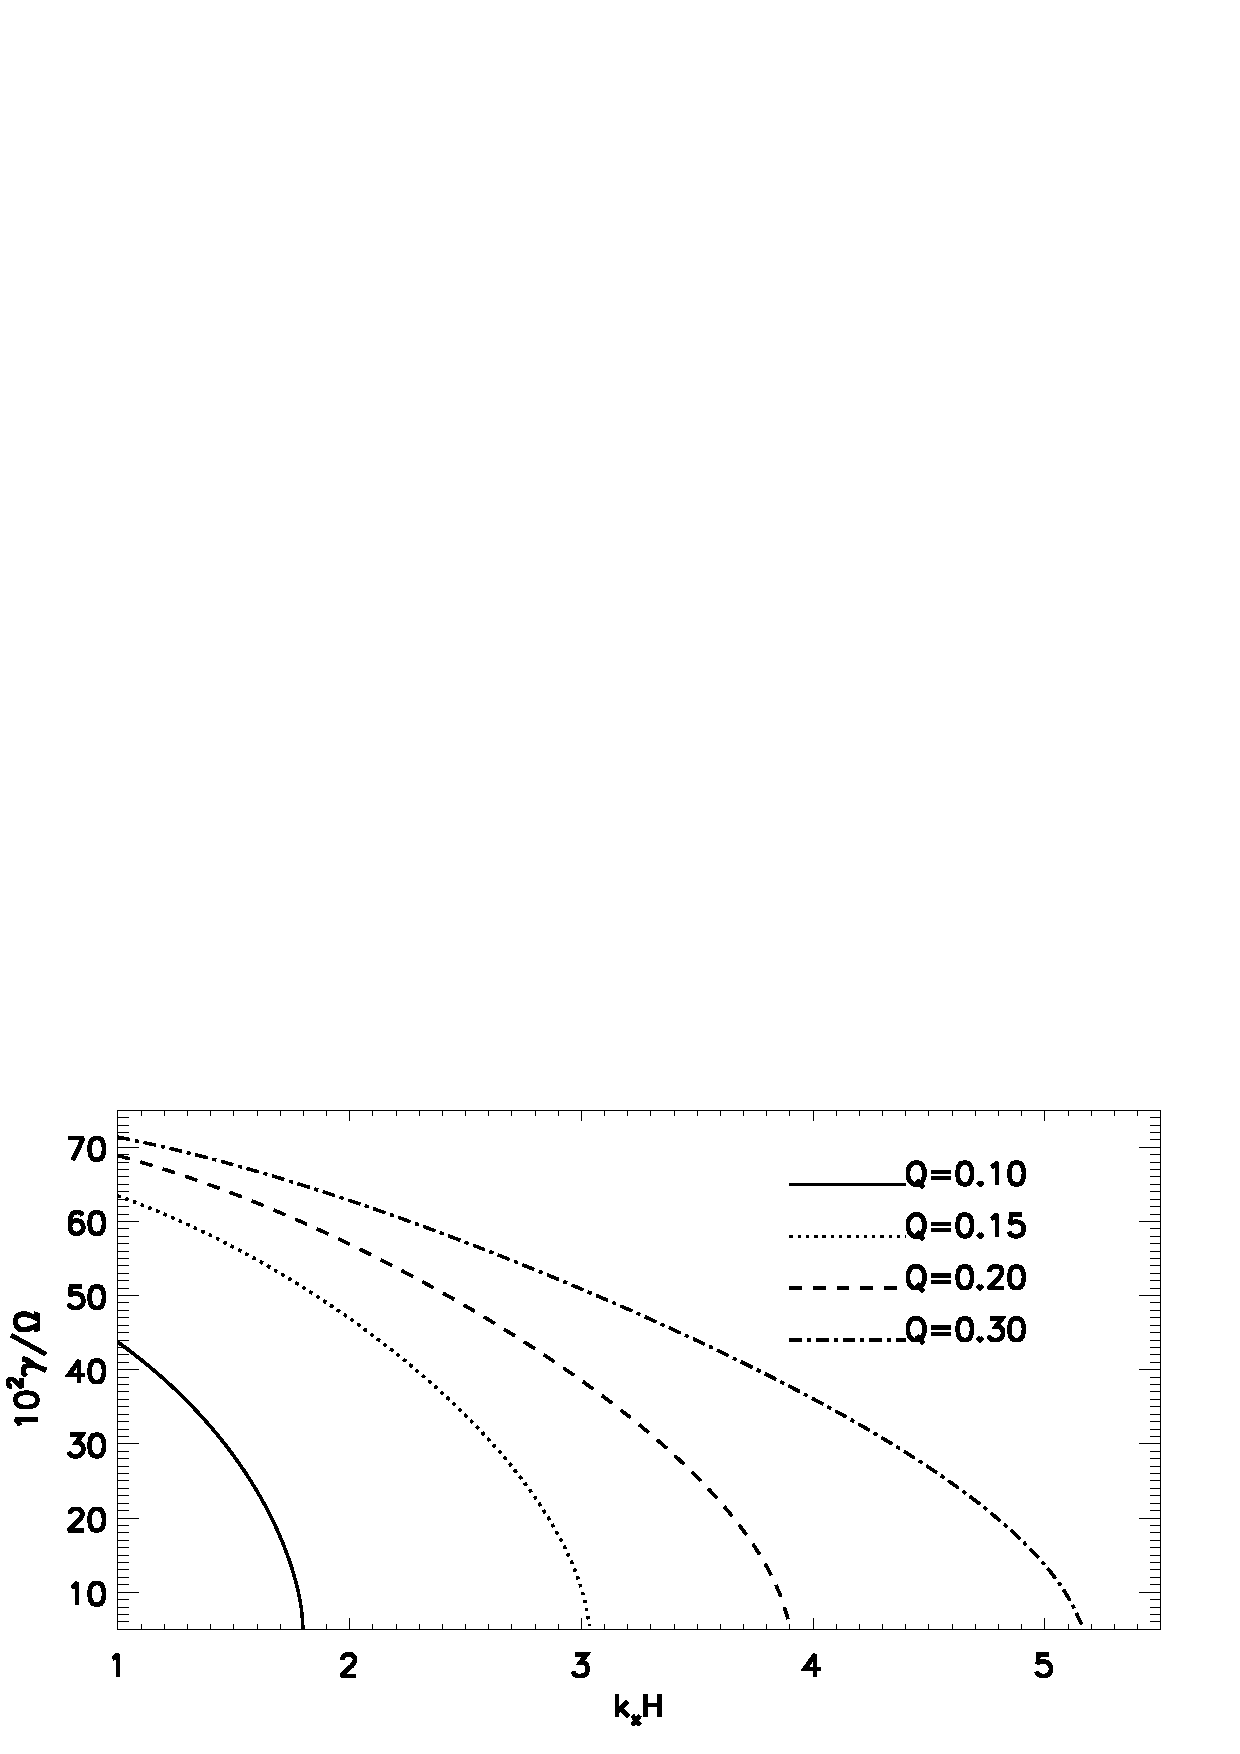
\includegraphics[width=\linewidth]{figures/compare_growth_poly_varQ_kx}
  \caption{MRI growth rates in self-gravitating polytropic disks, as a
    function of the horizontal wavenumber $k_x$. The disk is ideal
    ($\Lambda_0=10^2,\, A=1$) with $\beta = 40$. These modes have negligible
    density/potential perturbations.  
    \label{compare_growth_poly_kx}}
\end{figure}



\subsection{Influence of self-gravity on the MRI through the linear
  response}  
Our goal here is to examine whether or not self-gravity can amplify
the density perturbations associated with the MRI. We compute unstable modes
in a massive isothermal disk with $Q=0.2$ (corresponding to
$Q_\mathrm{2D}=0.72$), which is still expected to be marginally  
stable to gravitational instability \citep[][who find
a critical value of  $Q\simeq 0.2$]{mamat10}.   
The upper disk boundary is set to $Z_s=H$. 

%resolution Nz=256

\subsubsection{Ideal disks}
We first consider ideal MHD by adopting a uniform 
resistivity with $\Lambda_0=100$.  
Fig. \ref{gravity_energy} plots MRI growth rates as a function of
$k_x$ for several values of $\beta$. The curves are color-coded 
according $\tau$. (Recall $\tau\to1$ implies self-gravity dominates
over magnetic perturbations, and $\tau\to0$ is the opposite limit.)  
The potential perturbation is negligible for all cases when
$k_xH\lesssim 0.5$, since the MRI becomes incompressible as $k_x\to
0$.  

\begin{figure}
  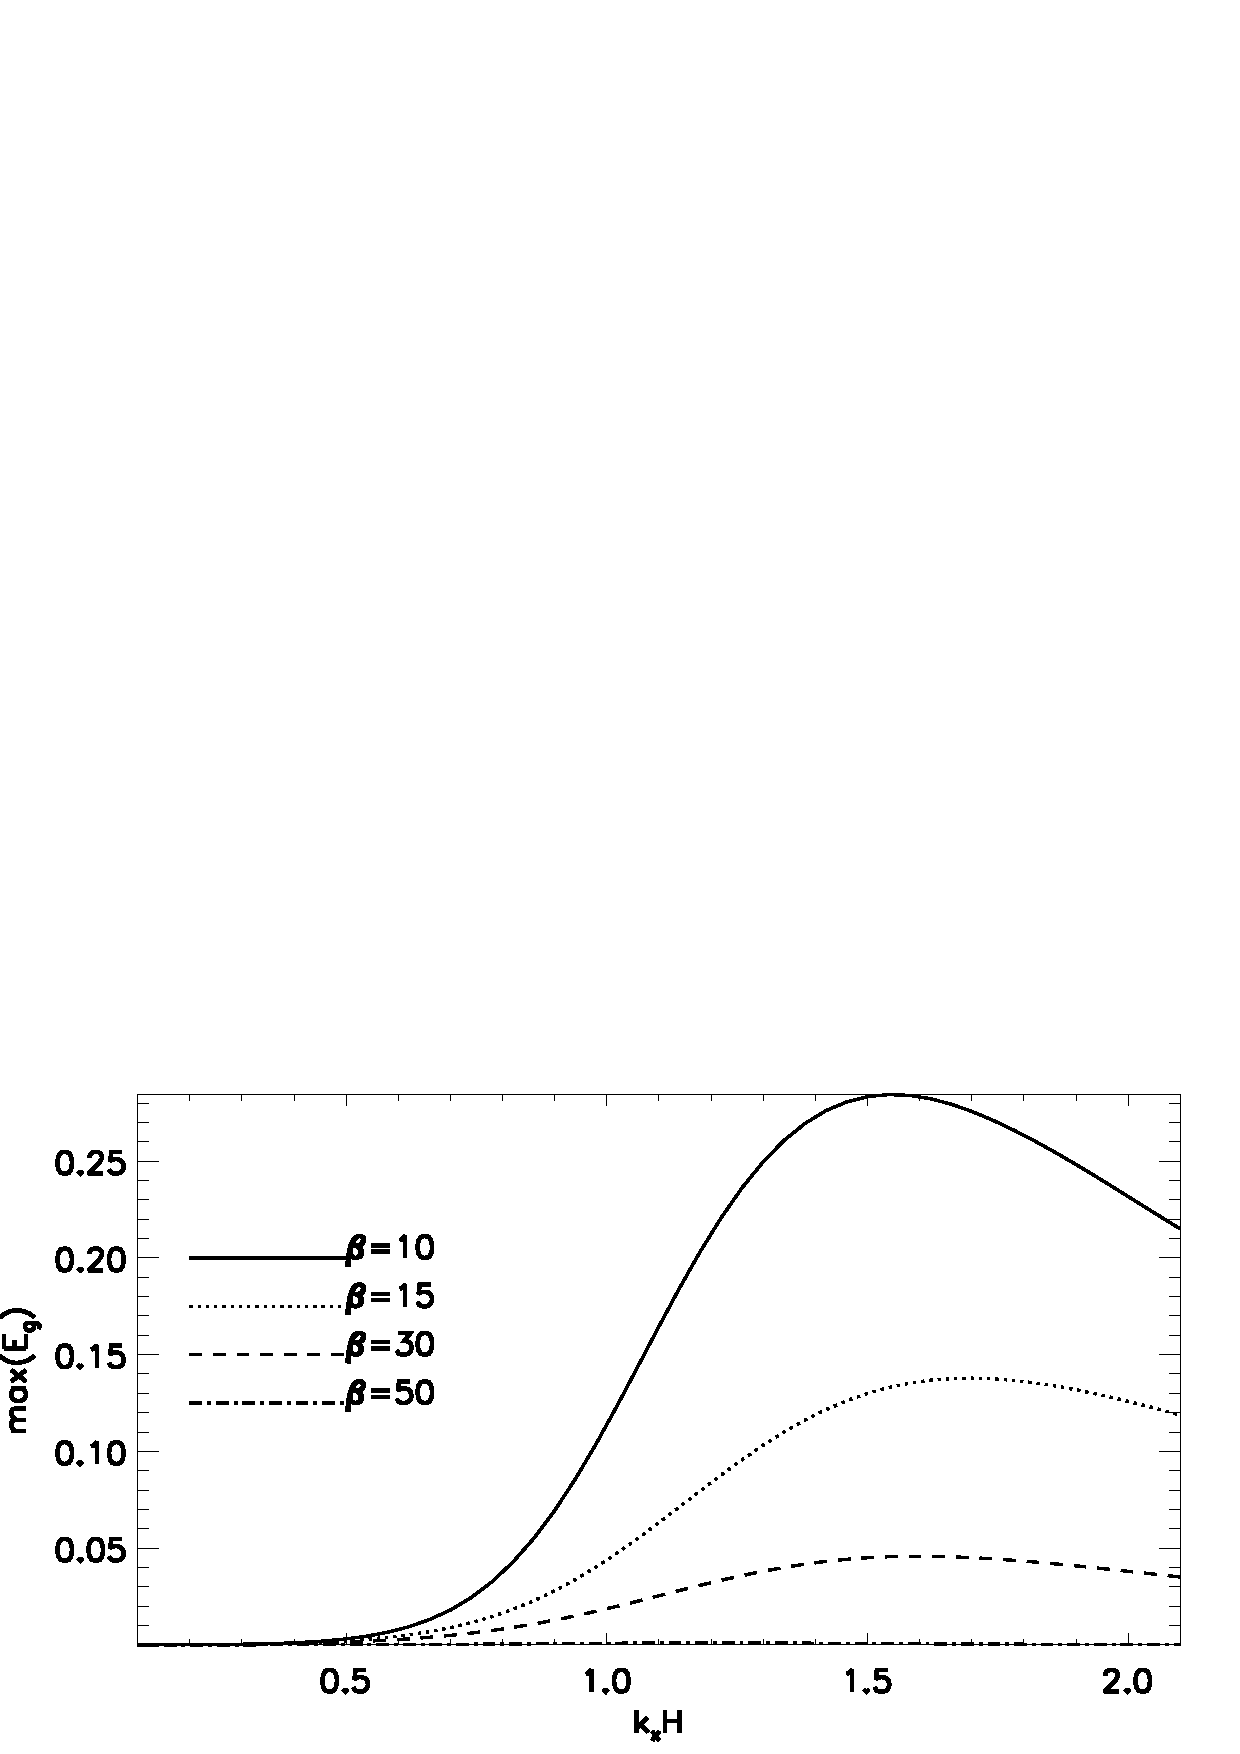
\includegraphics[width=\linewidth]{figures/compare_energy_ideal}
  \caption{Growth rates of MRI modes in isothermal self-gravitating
    disks with $Q=0.2$ ($Q_\mathrm{2D}=0.72$) in the limit of ideal MHD
    ($\Lambda_0=10^2$, $A=1$), for a range of field strengths $\beta$. The
    colorbar measures the importance of self-gravity by $\tau$.  
    %{\bf ADD BETA=8}
    \label{gravity_energy}}
\end{figure}

For $\beta\gg 1$, i.e. a weak field, density perturbations are
negligible and the incompressible MRI operates. However, as $\beta$ is
lowered and the MRI growth rate reduced, we find non-negligible
potential perturbation for $k_xH=O(1)$. This suggests that in a
strongly magnetized disk that still permits the MRI, the associated
density perturbation can be important when the disk is
self-gravitating. %but formall stable 



\subsubsection{Resistive disks}
We repeat the above calculation for resistive disks, but fix
$\beta=100$ and vary the midplane Elsasser number $\Lambda_0$. Growth
rates are shown in Fig. \ref{gravity_energy_resis}. 
Interestingly, the highly resistive case $\Lambda_0=0.1$ has
comparable magnetic and gravitational energies: at $k_xH\simeq1.3$ we
find $\tau\sim 0.3$, which corresponds to $\avg{E_g}\sim 0.5\avg{E_m}$.  
Fig. \ref{mri_massive_cowling} compares the magnetic
energy of this mode to that computed in the \emph{Cowling  
  approximation}, where the Poisson equation is ignored in the 
linearized equations and the potential perturbation set to zero  
(formally letting $Q\to\infty$ in Eq. \ref{lin_poisson}).  
The growth rate increases when self-gravity is included in the linear
response, since self-gravity is usually destabilizing. However, 
$\gamma$ and $E_m$ are very similar, indicating that the instability
in the self-gravitating calculation is fundamentally still the MRI.   

\begin{figure}
  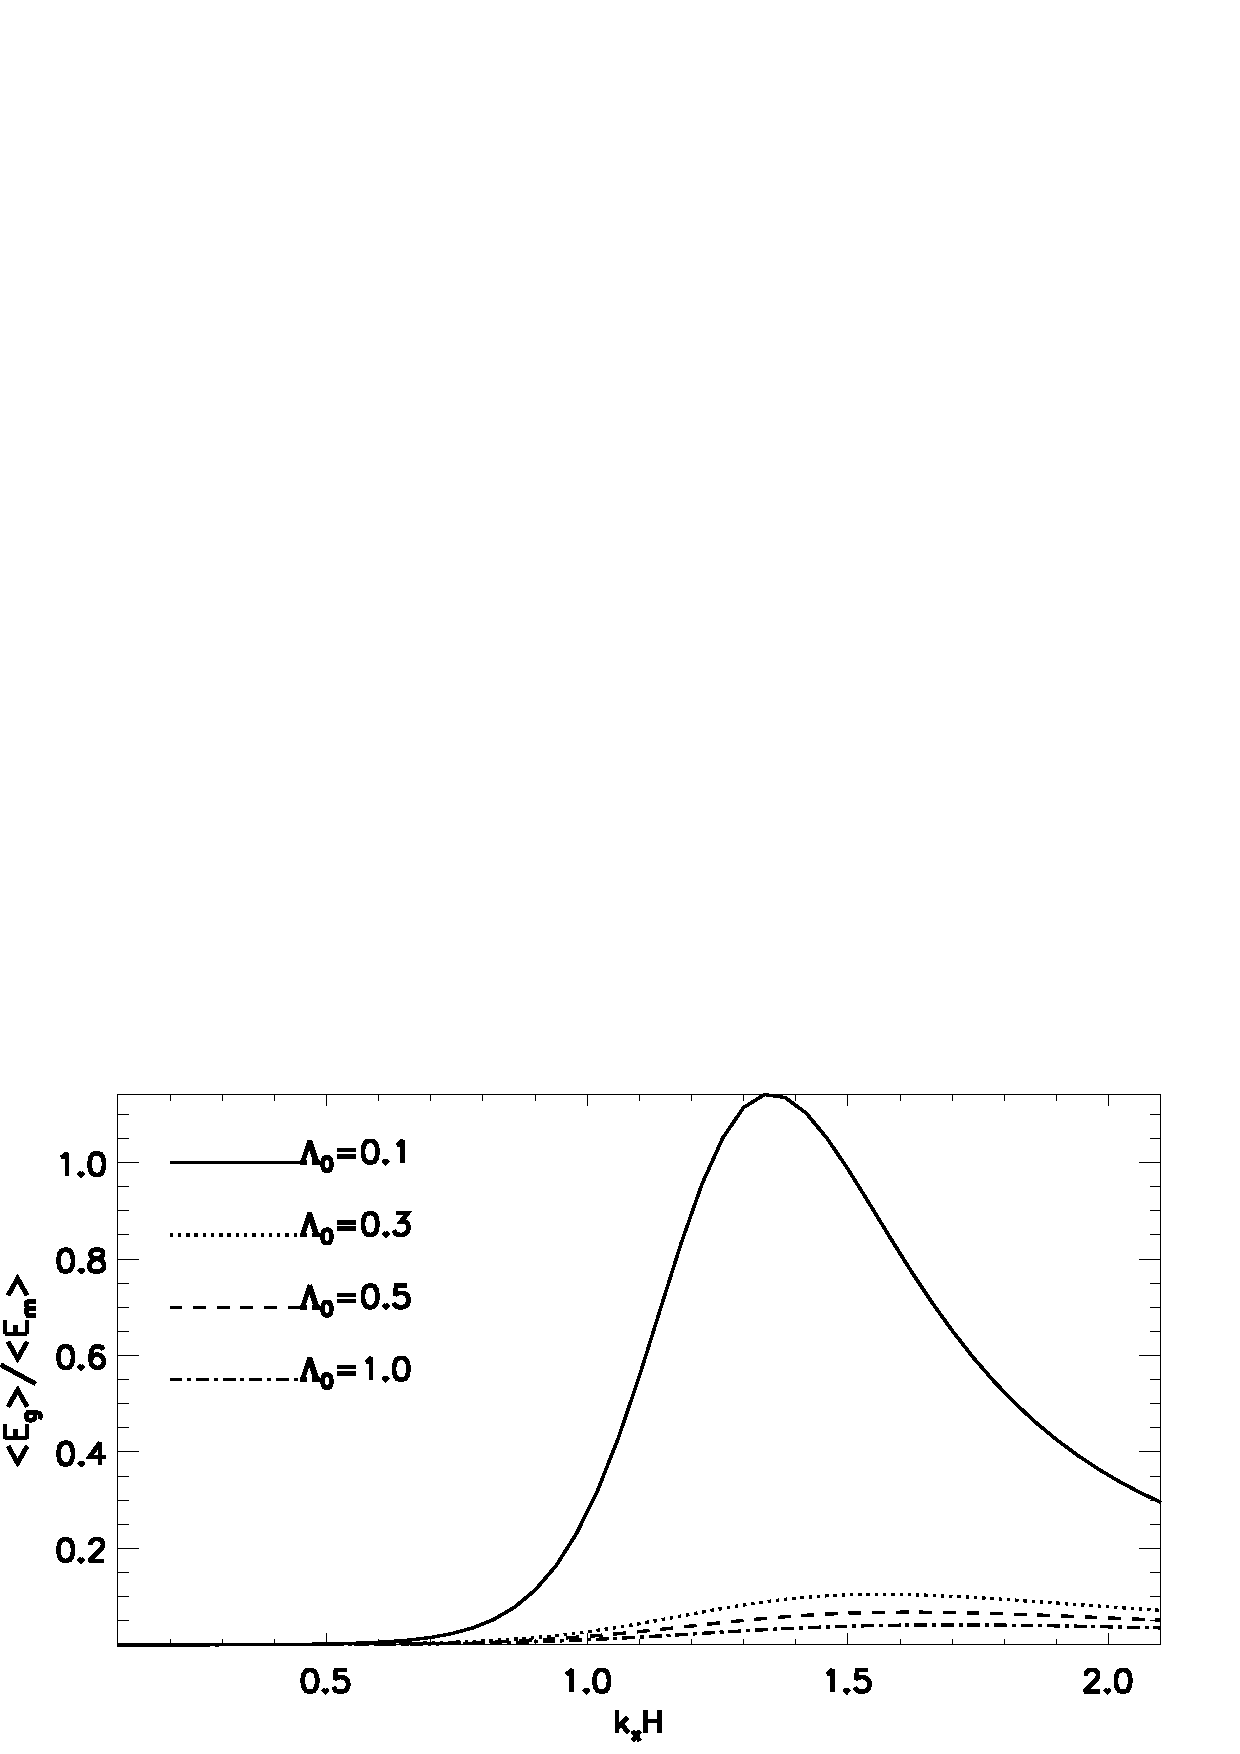
\includegraphics[width=\linewidth]{figures/compare_energy_resis}
  \caption{
    Growth rates of MRI modes in an isothermal self-gravitating
    disk with $Q=0.2$ ($Q_\mathrm{2D}=0.72$) at fixed $\beta=100$, 
    for a range of midplane Elsasser numbers. The resistivity is
    uniform. The colorbar measures the importance of self-gravity by $\tau$. 
    \label{gravity_energy_resis}}
\end{figure}


\begin{figure}
  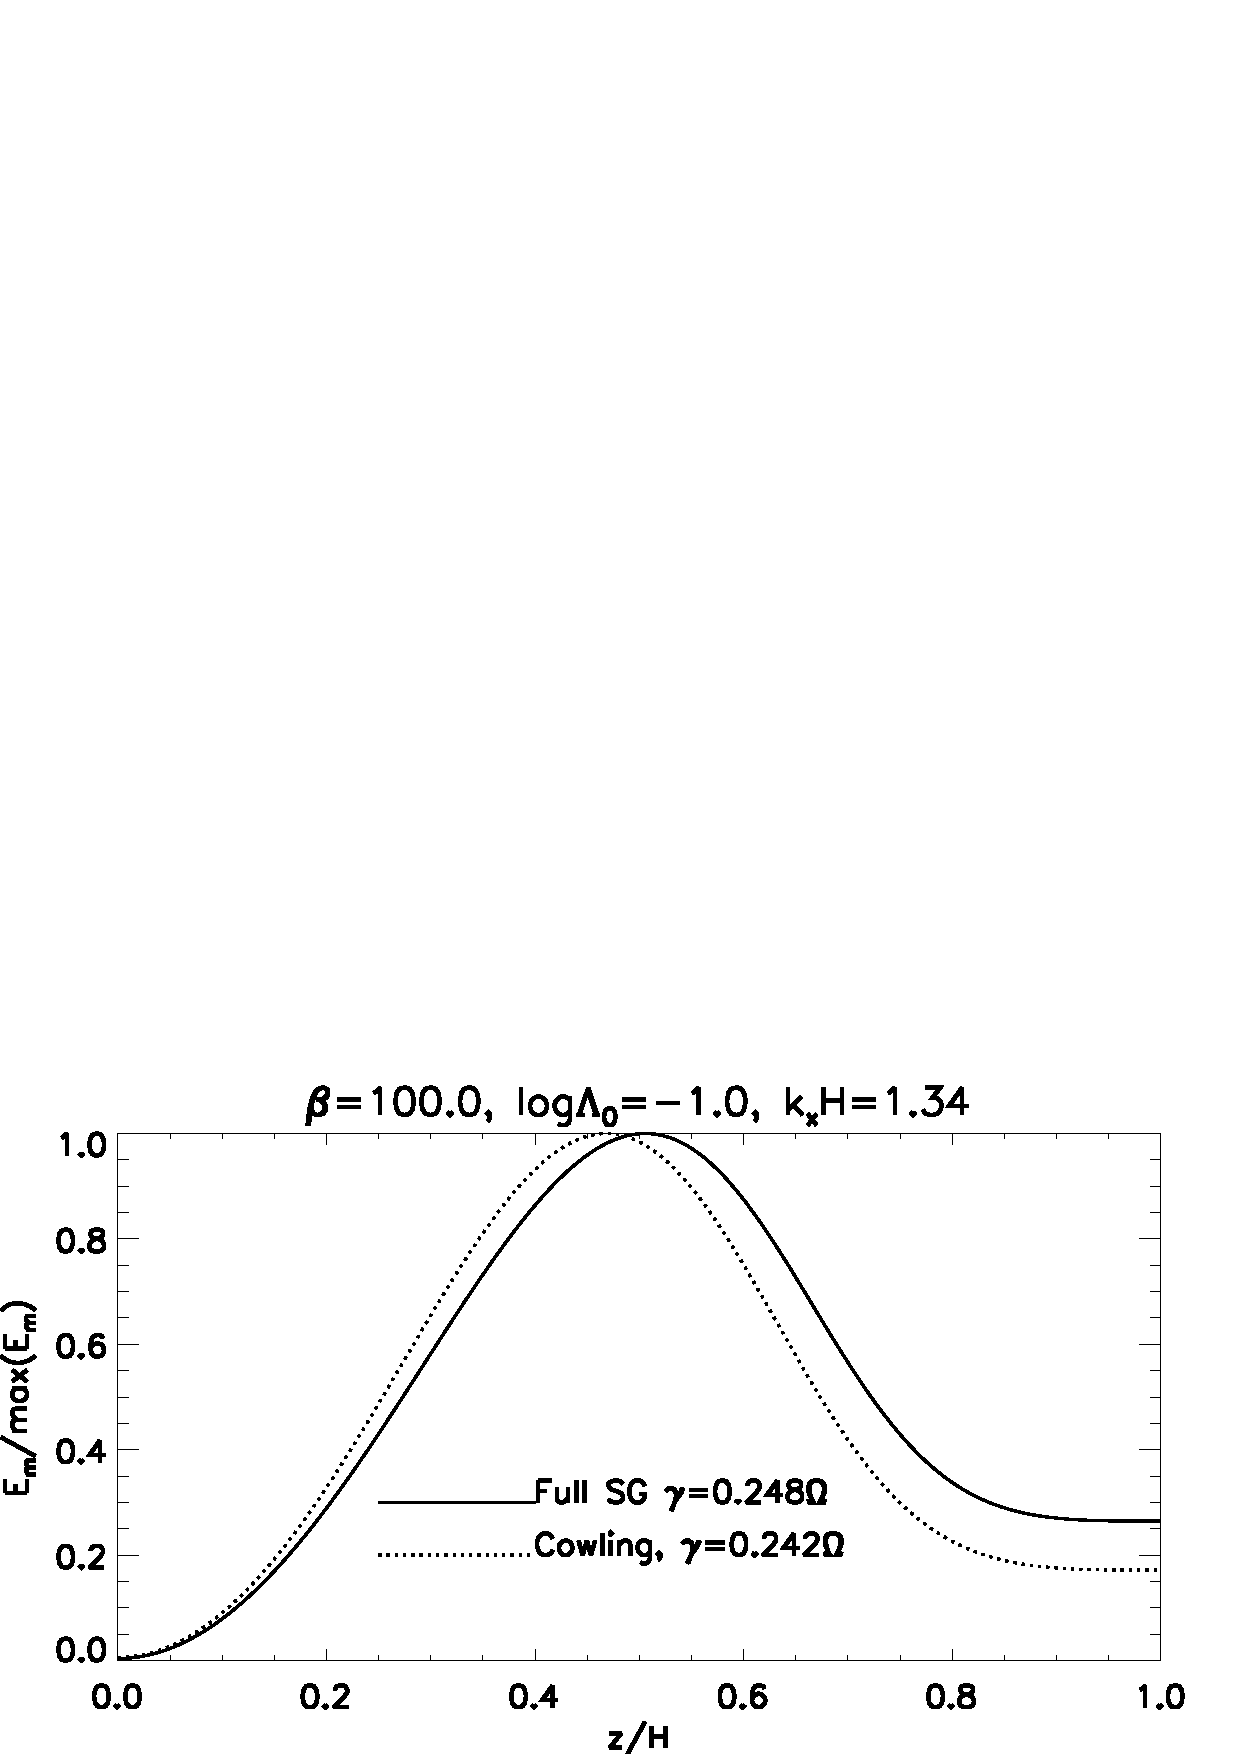
\includegraphics[width=\linewidth]{figures/compare_result_cowling}
  \caption{Magnetic energy associated with the linear mode with
    largest gravitational-to-magnetic energy ratio in 
    Fig. \ref{gravity_energy_resis} (solid) compared with that computed
    under the Cowling approximation (dotted). %{\bf REDO FIGURE}
    \label{mri_massive_cowling}}
\end{figure}

Fig. \ref{mri_massive_resis} plots the energies associated with the 
MRI mode discussed above. 
The gravitational energy exceeds the 
magnetic energy near the midplane ($z\lesssim0.2H$). The growth rate
$\gamma=0.25\Omega$ is not much smaller than that of the most unstable
mode ($\gamma=0.36\Omega$ for $k_xH=0.1$), so significant density
perturbations will grow on dynamical timescales for this
system, even though GI is not expected.

\begin{figure}
  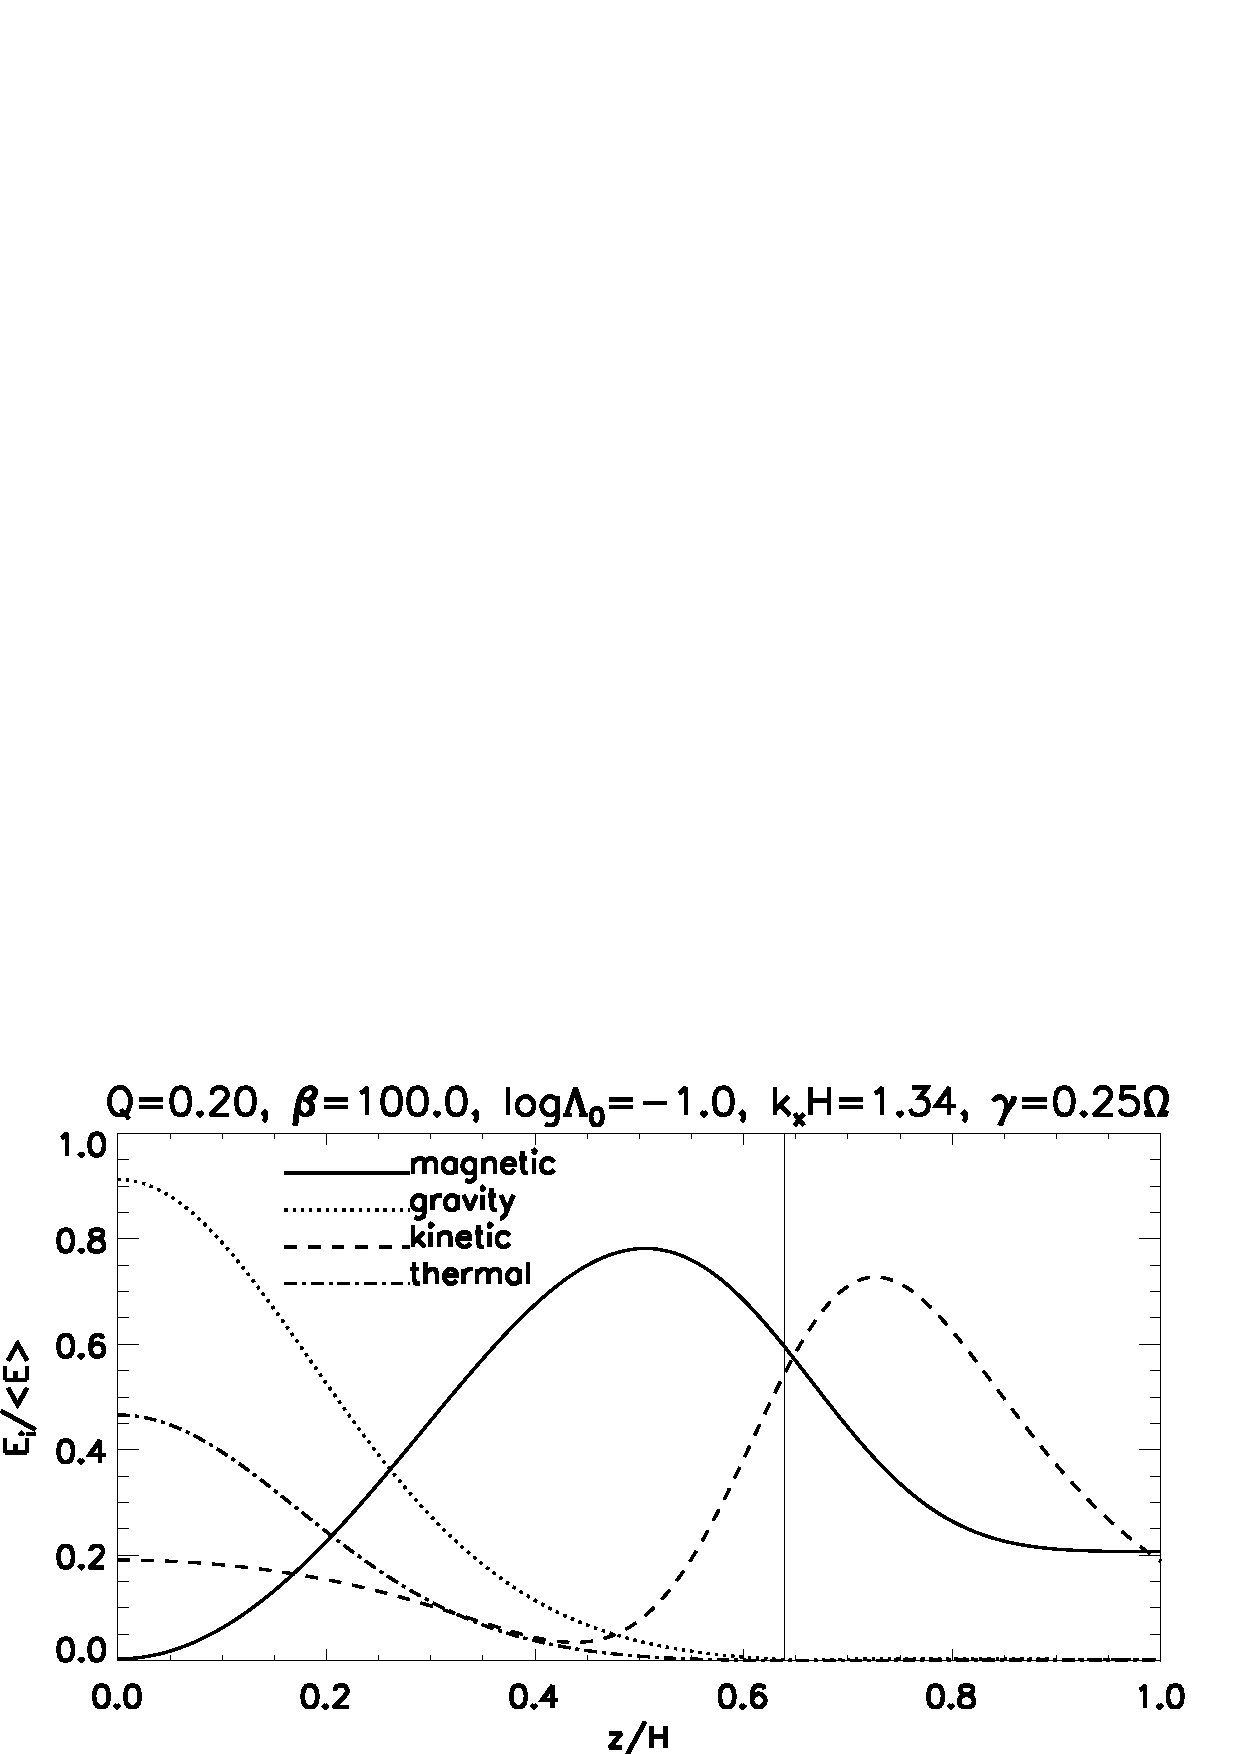
\includegraphics[width=\linewidth]{figures/result_resis_sg}
  \caption{Example of a resistive MRI mode with significant
    gravitational potential perturbation. The disk is isothermal. 
    The vertical line
    indicates $\Lambda=1$.  
    \label{mri_massive_resis}}
\end{figure}

\subsubsection{Qualitative interpretation} 
To make sense of the above results, we first return to ideal MHD and 
consider regions close to the disk midplane ($z\sim 0$), where
self-gravity is expected to be most important. For this discussion we
will ignore stratification and set $d^2/dz^2\to -k_z^2$. The governing
equations are then 

\begin{align}
  &  0= v_A^2k^2\dvx + \imgi\sigma\left(\imgi\sigma \dvx - 2\Omega\dvy + \imgi k_x \w\right),\label{simp1}\\
  &  0= v_A^2k_z^2\left(\dvy + \frac{\imgi S
  }{\sigma}\dvx\right) + \imgi\sigma\left(\imgi\sigma\dvy +
  \frac{\kappa^2}{2\Omega}\dvx\right),\label{simp2}\\
  & 0 = -k_z^2\w + \frac{\sigma^2}{c_s^2}W + \sigma k_x \dvx, \label{simp3}\\
  & 0 = k^2\dphi + \frac{\Omega^2}{c_s^2Q}W,\label{simp4}
\end{align}
where $k^2 = k_z^2 + k_x^2$. We imagine an iterative procedure to
solve the above equations, starting from the Cowling approximation
where $\delta\Phi\to0$ and $Q\to\infty$. This is the standard MRI and we denote the
solution as $\dvx^{(0)}$, $\dvy^{(0)}$ and $W^{(0)}$. Eq. \ref{simp3} implies
\begin{align}
  W^{(0)} = \frac{c_s^2\sigma k_x \dvx^{(0)}}{c_s^2k_z^2 - \sigma^2}. 
\end{align}
We argue below that $c_s^2k_z^2\gg \sigma^2$ by taking $k_z\sim
\Omega/v_A$. Then, recalling $W=c_s^2\delta\rho/\rho$, we can write
\begin{align}
  \frac{\delta\rho^{(0)}}{\rho} \sim
  \frac{\sigma}{\Omega}\frac{1}{\beta}\left[\frac{k_x\dvx^{(0)}}{\Omega}\right].   
\end{align}
The MRI has, in general, a non-zero density perturbation. However, it
is negligible for $k_x\to 0$ and/or a weak field ($\beta \gg 1$). 

% In general, the
%compressible MRI has $W^{(0)}\neq0$, since

We now include self-gravity.  The Poisson equation implies $W^{(0)}$
has an associated potential perturbation,     
\begin{align} 
  \dphi = -\frac{\Omega^2}{c_s^2 Q k^2} W^{(0)}.
\end{align}
Physically, we expect $k^2\geq0$, so that a positive (negative) local density
perturbation causes a negative (positive) local potential
perturbation. We then insert $\dphi$ back into the momentum and
continuity equations, and ask how does this potential perturbation
modify the Cowling solution? Writing $\dvx^{(0)} \to \dvx^{(0)} +
\dvx^{(1)}$ and similarly for $\dvy $ and $ W$, we find 


\begin{align}
  &   k_x\sigma \dphi = v_A^2k^2\dvx^{(1)} + \imgi\sigma\left[\imgi\sigma
  \dvx^{(1)} - 2\Omega\dvy^{(1)} + \imgi k_x W^{(1)}\right], \label{simp_pert1}\\ 
  &  0= v_A^2k_z^2\left[\dvy^{(1)} + \frac{\imgi S
    }{\sigma}\dvx^{(1)}\right] + \imgi\sigma\left[\imgi\sigma\dvy^{(1)} +
  \frac{\kappa^2}{2\Omega}\dvx^{(1)}\right],\label{simp_pert2}\\
  & k_z^2\dphi  = \left(\frac{\sigma^2}{c_s^2}-k_z^2\right)W^{(1)} +
  \sigma k_x \dvx^{(1)}.\label{simp_pert3} 
\end{align}
Now, if the perturbations to the magnetic field remain
unchanged, i.e. the mode remains close to the standard MRI as observed
in Fig. \ref{mri_massive_cowling}, then $\dvx^{(1)} \sim 0$ and
$\dvy^{(1)}\sim0$, so Eq. \ref{simp_pert2} is 
satisfied. Eq. \ref{simp_pert1} then require $\dphi +
W^{(1)}\sim0$. This is compatible with Eq. \ref{simp_pert3} if 
\begin{align}
  \left|k_z^2\right| \gg \left|\frac{\sigma^2}{c_s^2}\right|. \label{cond}
\end{align}
For the ideal MRI,  we take $k_z\sim \Omega/v_A$. Then
$|\sigma^2/c_s^2k_z^2|\sim |\sigma^2/\Omega^2\beta|\ll1$ because
$|\sigma|\lesssim \Omega$ and we are considering $\beta\gtrsim 10$. 
Thus Eq. \ref{cond} is generally satisfied.   

The above assumptions imply
\begin{align}
  W^{(1)} \sim \frac{\Omega^2}{c_s^2 Q k^2} W^{(0)},\label{feedback}
\end{align} 
which indicates a non-zero density perturbation due to the
MRI can be amplified by self-gravity. Now, for $k_xH\sim 1$ we have
$|k_z^2/k_x^2|\sim \beta/f^2\gg1$ because $f=O(1)$ and $\beta\gtrsim10$
for the cases considered above. Then
\begin{align}
  \left|\frac{W^{(1)}}{W^{(0)}}\right| \sim \frac{1}{Q\beta}, 
\end{align}
 suggesting stronger amplification of the density field by 
 self-gravity with increasing field strength (decreasing
 $\beta$). 

 

 The above arguments can be adapted to the resistive
 disk. Eq. \ref{simp3}---\ref{simp4} are unchanged, while resistive
 terms appearing in Eq. \ref{simp1}---\ref{simp2} only involve the
 potential perturbation through $\w$. For the resistive MRI we take
 $k_z\sim v_A/\eta$ and $|\sigma|\sim v_A^2/\eta = \Lambda\Omega$
 \citep{sano99}. Then $|\sigma^2/c_s^2k_z^2|\sim 1/\beta \ll 1$ so
 Eq. \ref{cond} is satisfied. Noting that $k_z^2\sim
 \Lambda^2\Omega^2\beta/c_s^2$, the feedback equation becomes
 \begin{align}
   \left|\frac{W^{(1)}}{W^{(0)}}\right| \sim
   \frac{1}{Q\left(f^2\hat{k}_x^2 + \beta\Lambda^2\right)},
 \end{align}
 so increasing the resistivity (decreasing $\Lambda$) should enhance
 density perturbations.  

%these arguments assume, of course, there is a non-zero density
%perturbation in the first place for self-gravity to ehance. 

 For weak fields in an ideal disk, the MRI has a vertical
 wavelength $\lambda \ll H$. It will be almost incompressible so the 
 `seed' density perturbation $W^{(0)}$ is small.  
 The perturbed mass contained within 
 $\sim \lambda$ is small and its potential is
 unimportant. Furthermore, considering the stratified  
 disk, $\lambda\ll H$ imply rapid variations in the density
 perturbation across the disk height, averaging to zero, so the
 magnitude of the associated potential perturbation is small. 
 Self-gravity does not affect the MRI in this regime.   
 
%the `seed' density pert is also small
%weak amplification

 However, a strong field and/or large resistivity increases the MRI
 vertical wavelength. When the vertical scale of the MRI becomes
 comparable to the disk thickness, i.e. $\lambda\sim H$, the
 perturbed mass across the disk height can contribute to a net potential
 perturbation. We therefore expect a necessary condition for
 self-gravity to affect the MRI is for the latter to be weak. 
%we are not considering GI yet

%Our
% interpretation above also assumes that the Cowling solution can
% provide some `seed' density perturbation. 
%Thus we also require the
% MRI to be compressible. 
%there has to be some  `seed' density perturbation provided by the
%non-SG MRI 

\section{Gravitationally unstable disks} \label{result2}
Gravitational instability becomes possible in a sufficiently
massive and/or cold disk. Here, we explore whether or not GI and MRI
can interact by computing unstable modes for isothermal disks with $Q < 0.2 $
($Q_\mathrm{2D}\lesssim ~0.67$) which permits GI, as shown below.
We consider ideal disks with $\Lambda_0=100$ and $A=1$, unless
otherwise stated.  

\subsection{Co-existence of MRI and GI} 
Fig. \ref{compare_growth3} show growth rates for modes with $k_xH=1$
as a function of $\beta$ in disks with $Q=0.18$, $Q=0.14$ and
$Q=0.12$.   
All three cases display distinct GI modes (red/brown branch). The GI 
growth rates are $\gamma\simeq 0.25\Omega,\,0.6\Omega,\,0.8\Omega$ for
$Q=0.18,\,0.14,\,0.12$, respectively. GI is stabilized by magnetic
pressure for sufficiently small $\beta$. The critical
field strength for stabilizing GI increases with increasing
self-gravity, consistent with \cite{nakamura83}.   
For $Q=0.18$, GI is stabilized for $\beta \lesssim 15$. Nevertheless, 
the MRI branch for $\beta < 15$ becomes self-gravitating, so that
density perturbations still grow, even though GI does not
formally operate.  

%critical beta increases with $Q$

\begin{figure}
  \includegraphics[width=\linewidth,clip=true,trim=0cm 2.1cm 0cm
    0cm]{figures/compare_growth3_kx1_Q0d18.ps} 
  \includegraphics[width=\linewidth,clip=true,trim=0cm 2.1cm 0cm
    0.5cm]{figures/compare_growth3_kx1_Q0d14.ps} 
  \includegraphics[width=\linewidth,clip=true,trim=0cm 0cm 0cm
    0.5cm]{figures/compare_growth3_kx1_Q0d12.ps} 
  \caption{Growth rates for modes with $k_xH=1$ in isothermal ideal
    disks with $Q=0.18$ (top), $Q=0.14$ (middle) and $Q=0.14$ (bottom). The
    colorbar measures the importance of  
    self-gravity by $\tau$.   
    \label{compare_growth3}}
\end{figure}

The GI and MRI branches only interact when their growth rates
are similar. This is seen in Fig. \ref{compare_growth3} for $Q=~0.18$
where the GI branch approaches a MRI branch at $\beta\simeq 25,\,
\gamma\simeq 0.2\Omega$. In fact, following the red curve to smaller
$\beta$ indicates GI transitions to MRI. The
`gaps' in the GI and MRI branches for $Q=0.18$ and $Q=0.12$ may be due
to the phenomenon of avoided crossing, as seen in stars
\citep[e.g.][]{aizenman77} and accretion tori
\citep[e.g.][]{christo93}, where physically distinct modes approach
one another in frequency and exchange character. However, we cannot
exclude the possibility  that some modes may have been missed in a 
numerical search of eigenfrequencies.  
%maybe ogilvie?

Thus, our results do not rigorously prove that the GI and MRI branches
do not intersect.  Nevertheless, the continuous variation of $\tau$
strongly suggest that unstable modes can transition smoothly from 
MRI to GI and vice versa, especially at low $\beta$.     
%no unique transition

\subsubsection{Case study} 
In reality, perturbations with a range of $k_x$ will be present for a
given set of disk parameters. Fig. \ref{compare_growth3_Q01d2} show
growth rates as a function of $k_x$ in a disk with
$Q=0.12,\,\beta=20$, where MRI and GI have comparable growth
rates. All perturbations with $k_xH \lesssim 3.5$ grow dynamically
($\gamma\gtrsim 0.1\Omega$, or $\lesssim$ 1.6 orbits).

We also plot in Fig. \ref{compare_growth3_Q01d2} growth rates obtained 
from the Cowling approximation, which isolates MRI; and that from a
high-resistivity run, which isolates GI by allowing the field lines to
slip through the fluid. We refer to these as  
pure MRI and pure GI, respectively.  
For $k_xH\lesssim 0.7$, growth rates are equal to
those on the pure MRI and pure GI branches. That is, MRI and GI
operate independently until their growth rates become equal as a
function of $k_x$.  

The dispersion relation $\gamma(k_x)$ deviates from the
pure GI/MRI curves with increasing $k_x$, implying stronger interaction between
magnetic and density perturbations. Comparing pure GI (dashed line)
and the gravitationally-dominated portions of $\gamma(k_x)$ shows that 
inclusion of magnetic field stabilizes high-$k_x$ pure GI. (Note also
the slight decrease in the most unstable $k_x$.) 
This stabilization is due to magnetic pressure \citep{lizano10}, which
is consistent with stabilizing the small wavelength GI only.    

Comparing pure MRI (solid line) and the magnetically-dominated
portions of $\gamma(k_x)$ show that self-gravity increases MRI growth
rates at large $k_x$. This effect is small but noticeable, which can
be used as a code test for non-linear simulations. Note that this
destabilization is through the linear response, rather 
than through the background stratification (which is stabilizing).  

%smooth transitions, mode exchange

\begin{figure}
  \includegraphics[width=\linewidth]{figures/compare_growth3_Q0d12_B20.ps}  
  \caption{Growth rates of unstable modes in the massive isothermal
    disk with $Q=0.12$ and $\beta=20$, as a function of the horizontal
    wavenumber $k_x$. The colorbar measures the importance of
    self-gravity by $\tau$. The solid line corresponds to MRI modes in the
    Cowling approximation. The dashed line corresponds to pure GI
    modes, obtained by including a high resistivity in the full
    problem. 
    \label{compare_growth3_Q01d2}}
\end{figure}


\section{Effect of an azimuthal field}
We now extend the previous investigation to disks with an azimuthal
field, so that $B_y\neq 0$. 

%cannot consider superthermal fields
%compressibility important f

%\subsection{}
 

\appendix
\section{Analytic equilibrium for the polytropic disk}\label{appen1}
For a polytropic disk with $P = K\rho^2$ the dimensional equilibrium equation to
be solved is 
\begin{align}
  0=\csmid^2\frac{d^2}{dz^2}\left(\frac{\rho}{\rho_0}\right) +
  \Omega_z^2 + \frac{\Omega^2}{Q}\left(\frac{\rho}{\rho_0}\right), 
\end{align}
which is obtained by combining Eq. \ref{eqm_eqns1} and
\ref{eqm_eqns2} with the above equation of state. The solution is
\begin{align}  
  \frac{\rho}{\rho_0} = \left(1 + \frac{\Omega_z^2}{\Omega^2}Q\right)\cos{\left(a z\right)} - 
  \frac{\Omega_z^2}{\Omega^2}Q,  
\end{align}
where  
\begin{align}
  a^2 \equiv \frac{\Omega^2}{Q\csmid^2}. 
\end{align}
The polytropic disk thickness is
\begin{align}
  H =
  \frac{\csmid}{\Omega}\sqrt{Q}\arccos\left(\frac{\Omega_z^2Q}{\Omega^2+ \Omega_z^2Q}\right).  
\end{align}
Given a fixed mid-plane temperature, the function $f(Q)\equiv
\csmid/\Omega H$ is an inverse measure of the disk thickness, and $f$ increases with decreasing $Q$,
as shown in Fig. \ref{plot_fq}. This corresponds to a thinner disk
with increasing strength of vertical self-gravity.

\begin{figure}
  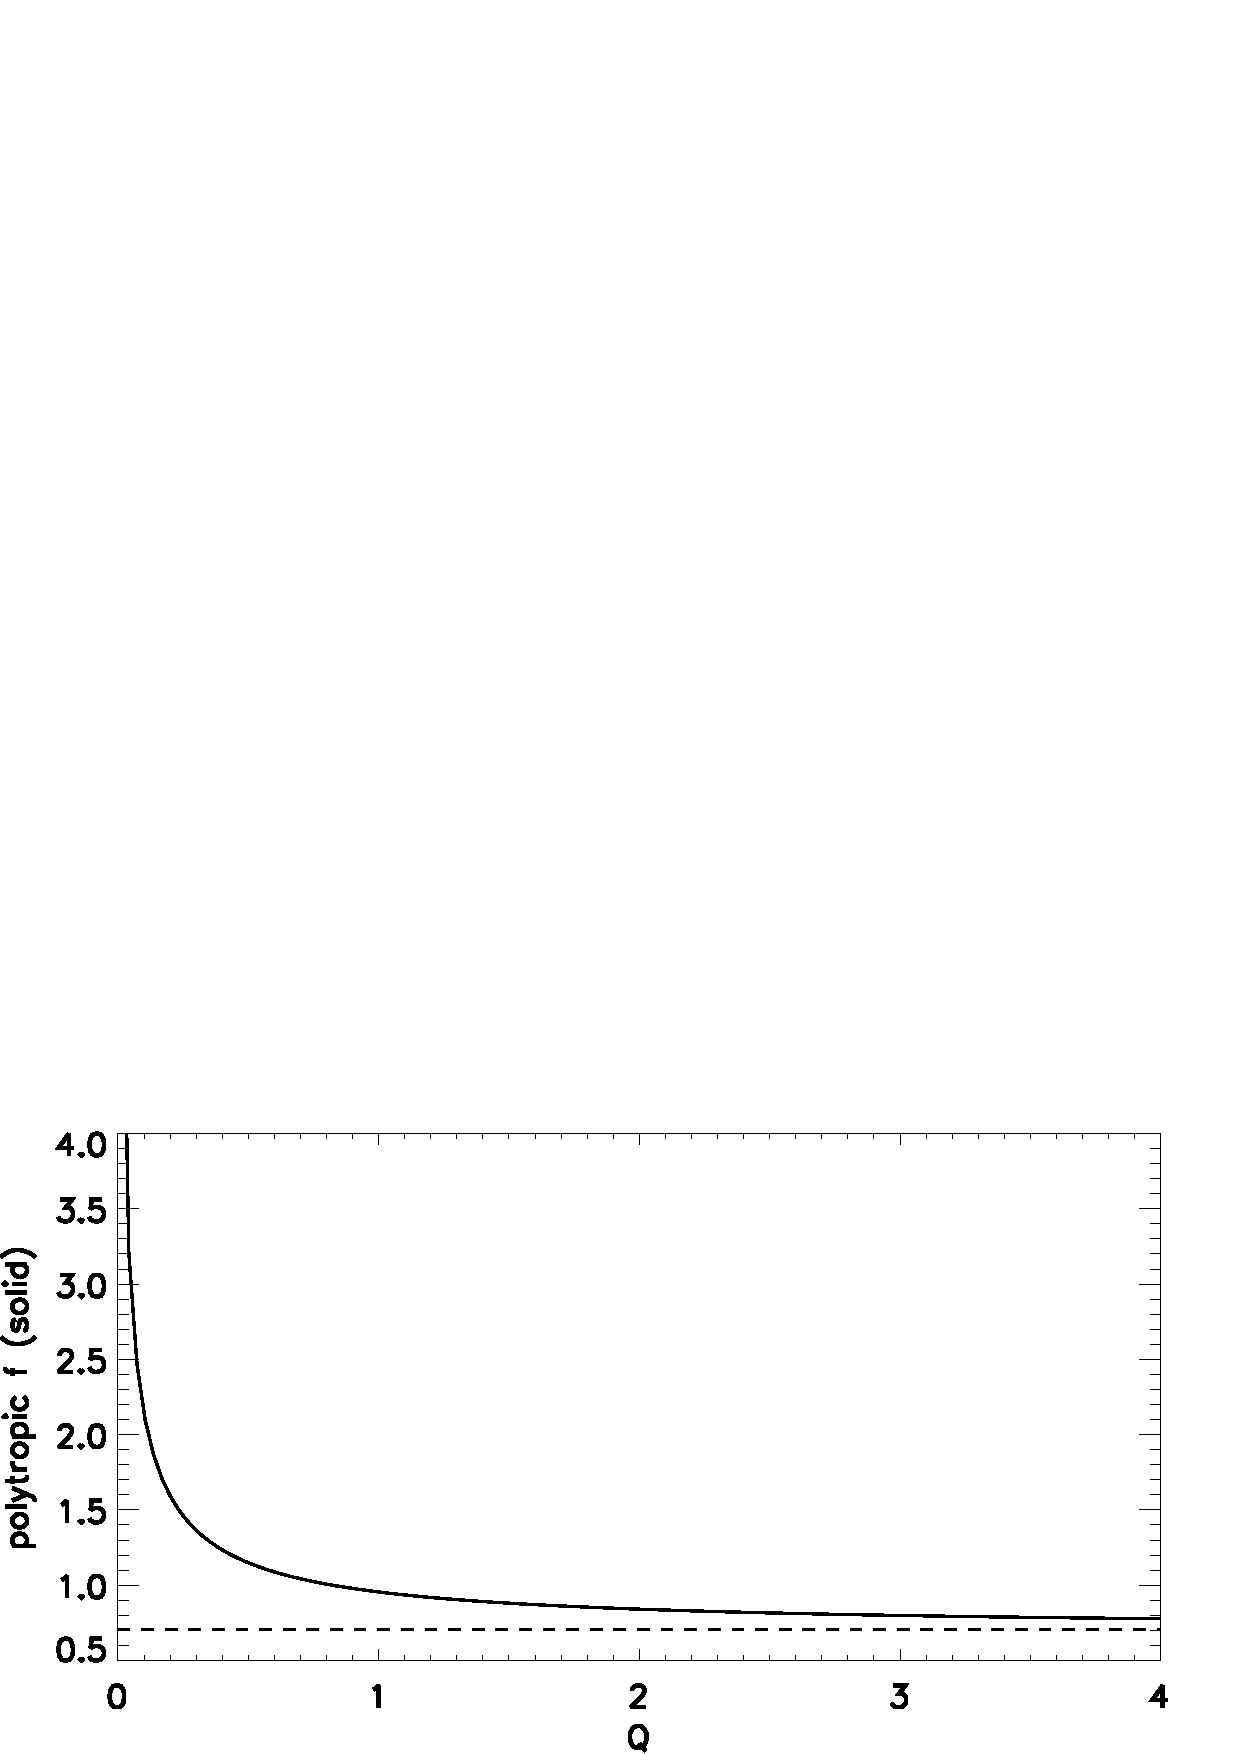
\includegraphics[width=\linewidth]{figures/plot_fq}
  \caption{The function $f(Q)$ describing vertical hydrodstatic 
    equilibrium in self-gravitating polytropic disks (solid line). The
    horizontal dashed line is the asymptotic value of $1/\sqrt{2}$ for
    large $Q$.  
    \label{plot_fq}}
\end{figure}

\section{Relation between $Q$ and the Toomre parameter}\label{q3d2d}
The Toomre parameter defined for razor-thin disks is 
\begin{align} 
  Q_\mathrm{2D}\equiv \frac{\kappa c_s}{\pi G\Sigma},  
\end{align}
where $\Sigma$ is the total column density. To relate our
self-gravity parameter $Q$ and $Q_\mathrm{2D}$, we replace $c_s$ by
$\overline{c_s}\equiv\int\rho c_s dz/\int\rho dz$, and 
$\kappa$ by $\Omega$, giving
\begin{align}
  Q_\mathrm{2D} = 2Qf \frac{\int_0^1
    \hat{\rho} \hat{c}_s
    d\hat{z}}{\left(\int_0^1 \hat{\rho} d\hat{z}\right)^2},   
\end{align}
where each term on the right-hand-side is non-dimensionalized (see
\S\ref{non-dim}). Fig. \ref{plot_q3d2d} plots this relation 
for isothermal and polytropic disks.  

\begin{figure}
  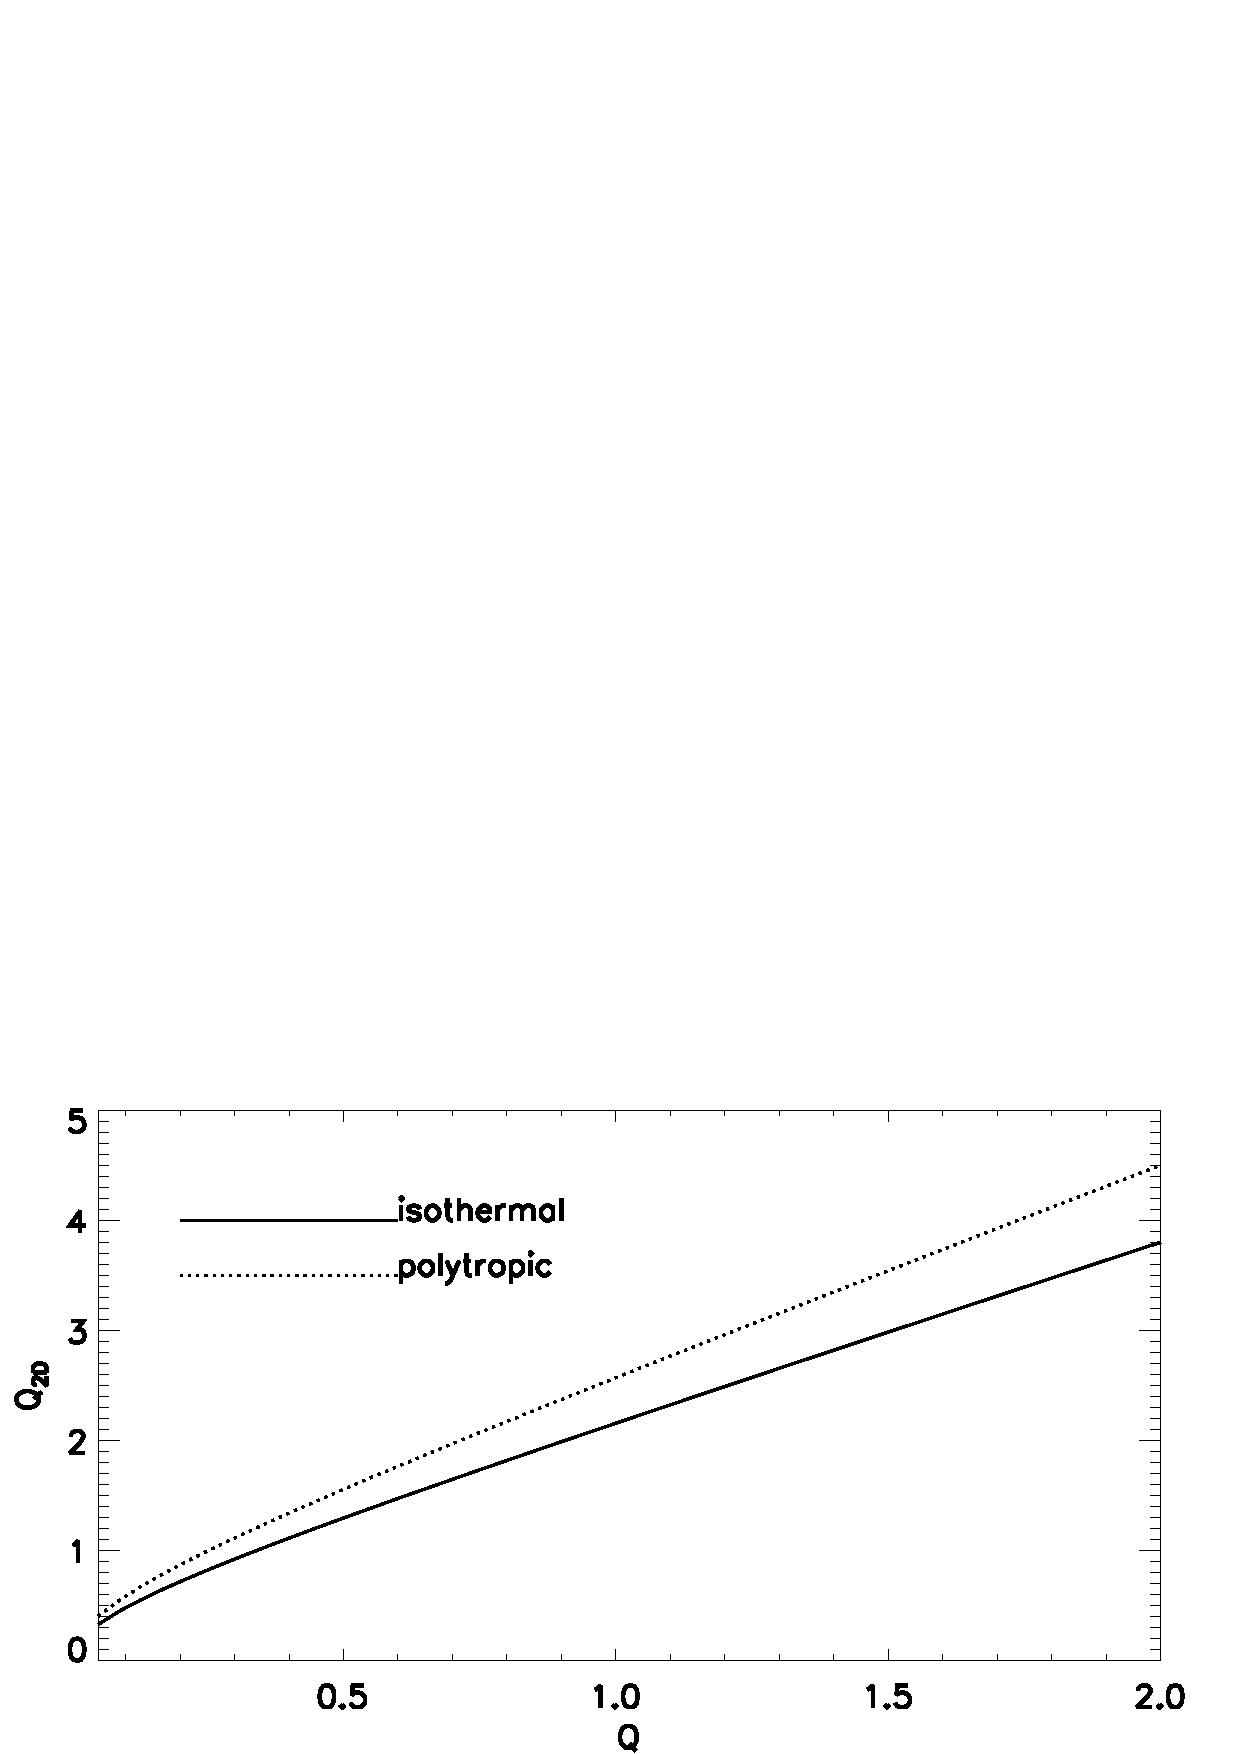
\includegraphics[width=\linewidth]{figures/q2d_iso}
  \caption{Relation between the self-gravity parameter $Q$ used in
    this paper and the Toomre parameter $Q_\mathrm{2D}$ for razor-thin
    disks. 
    \label{plot_q3d2d}}
\end{figure}


\section{Reduction to linear hydrodynamics}\label{reduction} 
Our task here is to remove the magnetic field and vertical velocity
perturbations from the linearized equations. Let us first define operators
\begin{align}
  D_0 = 1, \quad D_1 = \frac{\rho^\prime}{\rho} + \frac{d}{dz}, \quad
  D_2 = \frac{\rho^{\prime\prime}}{\rho} +
  \frac{2\rho^\prime}{\rho}\frac{d}{dz} + \frac{d^2}{d z^2},
\end{align}
and 
\begin{align}
  \overline{D}_0 = \eta D_0, \quad \overline{D}_1 = \eta^\prime D_0 + \eta
  D_1,\quad \overline{D}_2 = \eta^{\prime\prime} D_0 + 2\eta^\prime D_1 +
  \eta D_2. 
\end{align}
And we define the variables
\begin{align}
  &U \equiv \imgi\sigma\dvx - 2\Omega\dvy + \imgi k_x \w,\\
  &V \equiv \imgi\sigma\dvy + \frac{\kappa^2}{2\Omega}\dvx.
\end{align}

We first express the continuity equation in terms of horizontal
velocity, density and potential perturbations. 
The vertical velocity perturbation is 
\begin{align}
  \dvz = \frac{\imgi}{\sigma}\left(\w^\prime + \epsilon V\right),  
\end{align}
where the linearized $y$ momentum equation was used (i.e. eliminating
$\dby^\prime$ between Eq. \ref{lin_vy} and Eq. \ref{lin_vz}). 
Inserting this into the linearized continuity equation
(Eq. \ref{lin_cont}), we obtain
\begin{align}
0 = W^{\prime\prime} + \left(\ln{\rho}\right)^\prime W^\prime +
\frac{\sigma^2}{c_s^2}W +  \dphi^{\prime\prime} + \left(\ln{\rho}\right)^\prime \dphi^\prime
 + \sigma k_x \dvx + \epsilon D_1 V.
%  0=  W^{\prime\prime} + \left(\ln{\rho}\right)^\prime W^\prime +
%  \frac{1}{c_s^2f^2}\left(\frac{\rho}{Q} + \sigma^2\right)W +
% \left(\ln{\rho}\right)^\prime\dphi^\prime + k_x^2\dphi + \frac{\sigma
%    k_x}{f}\dvx.\label{final_w}
\end{align}

Next, we examine separately the cases of a vertical field with
variable resistivity and that of a tilted field with uniform
resistivity. (A similar procedure can be performed in
the general case of a tilted field with variable resistivity.) 

\subsection{Vertical field with variable resistivity}
First consider $\epsilon = 0$ and $\eta=\eta(z)$ in the linearized
equations. Denoting the $n^\mathrm{th}$ vertical derivative as $^{(n)}$, the
equations of motion give
\begin{align}
  &\dbx^{(n)} = \frac{\mu_0\rho}{B_z}D_{n-1}U + \imgi k_x \dbz^{(n-1)},\label{bx_eq}\\
  &\dby^{(n)} = \frac{\mu_0\rho}{B_z}D_{n-1}V,\label{by_eq}
\end{align}
for $n\geq1$. Differentiating the divergence-free condition for the magnetic
field gives
\begin{align}
  \imgi k_x \dbx^{\prime} + \dbz^{\prime\prime} = 0.   
\end{align}
We insert the expression for $\dbx^\prime$ from Eq. \ref{bx_eq} and the
expression for $\dbz^{\prime\prime}$ from the $z$ component of the
linearized induction equation (Eq. \ref{induct_vert}) to obtain
\begin{align}\label{bz_eq}
  -\sigma\dbz^{(n)} = k_x B_z \dvx^{(n)} + k_x\frac{\mu_0\rho}{B_z}\overline{D}_nU. 
\end{align}

%\subsection{Eliminating $\dbx$}
Inserting the above expressions for $\dbx^{\prime\prime}$,
$\dbx^\prime$ (Eq. \ref{bx_eq}) and $\dbz^\prime$  (Eq. \ref{bz_eq})
into the right-hand-side of the $x$-induction equation (Eq. \ref{induct_x} ) gives   
\begin{align}
  \imgi\sigma \dbx =
  B_z\dvx^\prime + \frac{\mu_0\rho}{B_z}\overline{D}_1U. \label{bx_expression}
\end{align}
($\bar{\sigma}\neq0$ has been assumed to obtain this.) We
differentiate this expression with respect to $z$ and eliminate the
resulting $\dbx^\prime$ using Eq. \ref{bx_eq}, to obtain
\begin{align}
%  0 = B_z\dvx^{\prime\prime} -
%  k_x^2B_z\dvx + \frac{\mu_0\rho}{B_z}\left(\overline{D}_2 - k_x^2 \overline{D}_0
%    - \imgi\sigma D_0\right)U. \label{final_vx} 
  0 = v_A^2\left(\dvx^{\prime\prime} -
  k_x^2\dvx\right) + \left(\overline{D}_2 - k_x^2 \overline{D}_0
    - \imgi\sigma D_0\right)U. \label{final_vx} 
\end{align}

%\subsection{Eliminating $\dby$}
We follow a similar procedure as above to remove $\dby$. 
We use Eq. \ref{bx_expression} and Eq. \ref{by_eq} to 
eliminate $\dbx,\dby^\prime$ and $\dby^{\prime\prime}$ from the
right-hand-side of the $y$-induction equation (Eq. \ref{induct_y}), 
%\begin{align}
%  &\imgi\bar{\sigma}\dby = f\dvy^\prime - \imgi
%  S\frac{\dbz^\prime}{k_x} +
%  \eta\dby^{\prime\prime}+\eta^\prime\dby^\prime.  
%\end{align}
%We can now insert expressions for the magnetic field derivatives using
%Eq. \ref{by_eq} and \ref{bz_eq} to obtain an expression for $\dby$, 
\begin{align}
  \imgi\bar{\sigma}\dby = B_z\dvy^\prime + \frac{\imgi S}{\sigma}\left(
    B_z\dvx^\prime + \frac{\mu_0\rho}{B_z}\overline{D}_1U\right) +
  \frac{\mu_0\rho}{B_z}\overline{D}_1V. \label{by_expression}
\end{align}
We differentiate this expression with respect to $z$, then eliminate 
$\dby$ and  $\dby^\prime$ from the left-hand-side of the resulting
expression using Eq. \ref{by_expression} and 
Eq. \ref{by_eq}, respectively. We obtain
\begin{align}
0 = v_A^2\left(\dvy^{\prime\prime} -
\frac{\sbar^\prime}{\sbar}\dvy^\prime\right)  
+ \frac{\imgi S v_A^2}{\sigma}\left(\dvx^{\prime\prime} -
\frac{\sbar^\prime}{\sbar}\dvx^\prime\right) + \frac{\imgi
  S}{\sigma}\left(\overline{D}_2 -
    \frac{\sbar^\prime}{\sbar}\overline{D}_1 \right)U 
+\left(\overline{D}_2 -
    \frac{\sbar^\prime}{\sbar}\overline{D}_1 - \imgi\sbar D_0 \right)V. \label{final_vy}
%0 = B_z\left(\dvy^{\prime\prime} -
%\frac{\sbar^\prime}{\sbar}\dvy^\prime\right)  
%+ \frac{\imgi S B_z}{\sigma}\left(\dvx^{\prime\prime} -
%\frac{\sbar^\prime}{\sbar}\dvx^\prime\right) + \frac{\imgi
%  S}{\sigma}\frac{\mu_0\rho}{B_z} \left(\overline{D}_2 -
%    \frac{\sbar^\prime}{\sbar}\overline{D}_1 \right)U 
%+\frac{\mu_0\rho}{B_z} \left(\overline{D}_2 -
%    \frac{\sbar^\prime}{\sbar}\overline{D}_1 - \imgi\sbar D_0 \right)V. \label{final_vy}
%
%  0 =& \frac{f^2}{\beta\rho}\left(\dvy^{\prime\prime} -
%  \frac{\bar{\sigma}^\prime}{\bar{\sigma}}\dvy^\prime\right) 
%  + \sbar\sigma D_0\dvy  + \frac{\imgi 
%    S}{\sigma}\frac{f^2}{\beta\rho}\left(\dvx^{\prime\prime} -
%    \frac{\sbar^\prime}{\sbar}\dvx^\prime\right) -
%    \frac{\imgi\sbar\kappa^2}{2}D_0\dvx \notag\\
%    & + \left(\overline{D}_2 -
%    \frac{\sbar^\prime}{\sbar}\overline{D}_1\right)\left[\imgi\left(\sigma
%      - \frac{2S}{\sigma}\right)\dvy + \left(\frac{\kappa^2}{2} -
%      S\right)\dvx - \frac{Sfk_x}{\sigma}\w\right]. \label{final_vy}
\end{align}

Eq. \ref{final_vx} and \ref{final_vy} constitutes the first two
linearized equations to be solved.

\subsection{Tilted field with uniform resistivity}
Here we allow $\epsilon\neq 0$ but take $\eta$ to be constant. We
first obtain expressions for $\dbx$ and $\dby$. Differentiating
the $x$ momentum equation and replacing the resuting $\dbz^\prime$
using the divergence-free condition and $\dby^\prime$ using the $y$
momentum equation, we obtain an expression for $\dbx^{\prime\prime}$
which can be inserted into the $x$ induction equation. This gives
\begin{align}
  \imgi\sigma\dbx = B_z\dvx^\prime +
  \frac{\eta\mu_0\rho}{B_z}\left( D_1 U + \imgi\epsilon k_x D_0
  V\right).\label{bx_tilted}  
\end{align}
We can insert this into the $y$ induction equation to obtain
\begin{align}
  \imgi\sbar\dby = -B_y\Delta + B_z\dvy^\prime + \frac{\imgi
    S}{\sigma}\left[ B_z \dvx^\prime+ \frac{\eta\mu_0\rho}{B_z}\left( D_1 U + \imgi\epsilon k_x D_0
  V\right)\right] + \frac{\eta\mu_0\rho}{B_z}D_1V,\label{by_tilted}
\end{align} 
where we have also used the derivative of the $y$ momentum equation to
eliminate  $\dby^{\prime\prime}$. Recall $\Delta \equiv i k_x \dvx +
\dvz^\prime$, so that
\begin{align}
  \Delta = \imgi k_x \dvx + \frac{i}{\sigma}\left(\w^{\prime\prime} +
  \epsilon V^\prime\right) = -\left[\frac{\imgi\sigma W}{c_s^2} +
    \frac{\imgi\left(\ln{\rho}\right)^\prime}{\sigma}\left(\w^\prime +
    \epsilon V\right)\right], 
\end{align}
where the second equality results from the continuity equation. 

Now consider
\begin{align}
  \dbx^\prime - \imgi k_x \dbz = \frac{\mu_0\rho}{B_z}D_0U +
  \imgi\epsilon k_x \dby = \frac{\sigma}{\sbar}\dbx^\prime +
  \frac{\imgi k_x^2B_z}{\sbar}\dvx,
\end{align}
where the first equality corresponds to the $x$ momentum equation and
the second equality results from replacing $\dbz$ using the $z$
induction equation. We can now use the above expressions for $\dbx$
and $\dby$ (Eq. \ref{bx_tilted}--\ref{by_tilted}) to obtain
\begin{align}
0 = &v_A^2\left[k_x^2\left(1+\epsilon^2\right)\dvx - \frac{\epsilon k_x
  S}{\sigma}\dvx^\prime - \dvx^{\prime\prime}\right] + \imgi\epsilon
k_x v_A^2 \dvy^\prime + \frac{\epsilon^2 k_x
  v_A^2}{\sigma}\left(\w^{\prime\prime} + \epsilon V^\prime\right) 
\notag\\ &-\left[\eta\left(D_2 + \frac{\epsilon k_x S}{\sigma}D_1\right) -
  \imgi\sbar D_0 \right]U %\notag\\
- \frac{\imgi\epsilon^2k_x^2S}{\sigma}\eta D_0V.
\end{align}
%We can now use the above expression for $\dbx,\dby$ to eliminate
%$\dbx^\prime$ and $\$ in the $x$ momentum equation  
%\begin{align}
%  \dbx^\prime - \imgi k_x\dbz = \frac{}{}
%\end{align}

Similarly, we differentiate Eq. \ref{by_tilted} and use the $y$
momentum equation to eliminate $\dby^\prime$ to obtain
\begin{align}
0 = &v_A^2\dvy^{\prime\prime} + \frac{\imgi S}{\sigma}v_A^2
\dvx^{\prime\prime} +\frac{\imgi S}{\sigma}\eta D_2U +
\left\{\eta\left(D_2 - \frac{\epsilon k_x S}{\sigma} D_1\right) +
  \imgi\left[\frac{\epsilon^2v_A^2\left(\ln{\rho}\right)^{\prime\prime}}{\sigma}
    - \sbar\right]D_0\right\}V \notag\\ &+ \imgi\epsilon
  v_A^2\left\{\frac{\sigma}{c_s^2}\left[W^\prime -
    \left(\ln{c_s^2}\right)^\prime W\right] +
    \frac{1}{\sigma}\left[\left(\ln{\rho}\right)^\prime(\w^{\prime\prime}
      + \epsilon V^\prime)
      +\left(\ln{\rho}\right)^{\prime\prime}\w^{\prime} \right]\right\}.    
\end{align}

%\subsection{Non-dimensionalization}
%In practice we solve the linearized equations in non-dimensional form,
%by defining
%We further write 
%\begin{align}
%  &z=\hat{z}H,\quad k_x =  \hat{k}_x/H,\quad \sigma = \hat{\sigma}\Omega,
%  \quad \delta\bm{v} = \csmid 
%  \delta\hat{\bm{v}}, \\ 
%  &\delta\bm{B} = B\delta\hat{\bm{B}},\quad
%  \delta\rho = \rho\hat{W}/\hat{c}_s^2,\quad \delta\Phi =
%  \csmid^2\delta\hat{\Phi}, 
%\end{align}
%where we have introduced the non-dimensional enthalpy perturbation
%$\hat{W}$ and the sound-speed $\hat{c}_s=\csmid^{-1}\sqrt{dP/d\rho}$ can be 
%obtained from the equation of state. The background frequencies are
%written $S=\hat{S}\Omega$ and $\Omega_z=\hat{\Omega}_z\Omega$ and the 
%resistivity as $\eta = \hat{\eta}H^2\Omega$. 

%We will now drop the $\hat{\phantom{a}}$ notation. Henceforth it is
%understood that all variables have been appropriately normalized
%(i.e. $\Omega\to 1$ and $H\to 1$), unless otherwise stated.


%tilted field
% calculate b field vertical derivatives carefully
% try no velocity pert at bc
% try anti-aligned field 


\bibliographystyle{apj}
\bibliography{ref}


\end{document}

